\documentclass[a4paper]{article}

\def\npart {IB}
\def\nterm {Lent}
\def\nyear {2016}
\def\nlecturer {O. Randal-Williams}
\def\ncourse {Groups, Rings and Modules}
\def\nlectures {MWF.12}
\def\nnotready {}

% Imports
\ifx \nextra \undefined
  \usepackage[pdftex,
    hidelinks,
    pdfauthor={Dexter Chua},
    pdfsubject={Cambridge Maths Notes: Part \npart\ - \ncourse},
    pdftitle={Part \npart\ - \ncourse},
  pdfkeywords={Cambridge Mathematics Maths Math \npart\ \nterm\ \nyear\ \ncourse}]{hyperref}
  \title{Part \npart\ - \ncourse}
\else
  \usepackage[pdftex,
    hidelinks,
    pdfauthor={Dexter Chua},
    pdfsubject={Cambridge Maths Notes: Part \npart\ - \ncourse\ (\nextra)},
    pdftitle={Part \npart\ - \ncourse\ (\nextra)},
  pdfkeywords={Cambridge Mathematics Maths Math \npart\ \nterm\ \nyear\ \ncourse\ \nextra}]{hyperref}

  \title{Part \npart\ - \ncourse \\ {\Large \nextra}}
\fi

\author{Lectured by \nlecturer \\\small Notes taken by Dexter Chua}
\date{\nterm\ \nyear}

\usepackage{alltt}
\usepackage{amsfonts}
\usepackage{amsmath}
\usepackage{amssymb}
\usepackage{amsthm}
\usepackage{booktabs}
\usepackage{caption}
\usepackage{enumitem}
\usepackage{fancyhdr}
\usepackage{graphicx}
\usepackage{mathtools}
\usepackage{microtype}
\usepackage{multirow}
\usepackage{pdflscape}
\usepackage{pgfplots}
\usepackage{siunitx}
\usepackage{tabularx}
\usepackage{tikz}
\usepackage{tkz-euclide}
\usepackage[normalem]{ulem}
\usepackage[all]{xy}

\pgfplotsset{compat=1.12}

\pagestyle{fancyplain}
\lhead{\emph{\nouppercase{\leftmark}}}
\ifx \nextra \undefined
  \rhead{
    \ifnum\thepage=1
    \else
      \npart\ \ncourse
    \fi}
\else
  \rhead{
    \ifnum\thepage=1
    \else
      \npart\ \ncourse\ (\nextra)
    \fi}
\fi
\usetikzlibrary{arrows}
\usetikzlibrary{decorations.markings}
\usetikzlibrary{decorations.pathmorphing}
\usetikzlibrary{positioning}
\usetikzlibrary{fadings}
\usetikzlibrary{intersections}
\usetikzlibrary{cd}

\newcommand*{\Cdot}{\raisebox{-0.25ex}{\scalebox{1.5}{$\cdot$}}}
\newcommand {\pd}[2][ ]{
  \ifx #1 { }
    \frac{\partial}{\partial #2}
  \else
    \frac{\partial^{#1}}{\partial #2^{#1}}
  \fi
}

% Theorems
\theoremstyle{definition}
\newtheorem*{aim}{Aim}
\newtheorem*{axiom}{Axiom}
\newtheorem*{claim}{Claim}
\newtheorem*{cor}{Corollary}
\newtheorem*{defi}{Definition}
\newtheorem*{eg}{Example}
\newtheorem*{fact}{Fact}
\newtheorem*{law}{Law}
\newtheorem*{lemma}{Lemma}
\newtheorem*{notation}{Notation}
\newtheorem*{prop}{Proposition}
\newtheorem*{thm}{Theorem}

\renewcommand{\labelitemi}{--}
\renewcommand{\labelitemii}{$\circ$}
\renewcommand{\labelenumi}{(\roman{*})}

\let\stdsection\section
\renewcommand\section{\newpage\stdsection}

% Strike through
\def\st{\bgroup \ULdepth=-.55ex \ULset}

% Maths symbols
\newcommand{\bra}{\langle}
\newcommand{\ket}{\rangle}

\newcommand{\N}{\mathbb{N}}
\newcommand{\Z}{\mathbb{Z}}
\newcommand{\Q}{\mathbb{Q}}
\renewcommand{\H}{\mathbb{H}}
\newcommand{\R}{\mathbb{R}}
\newcommand{\C}{\mathbb{C}}
\newcommand{\Prob}{\mathbb{P}}
\renewcommand{\P}{\mathbb{P}}
\newcommand{\E}{\mathbb{E}}
\newcommand{\F}{\mathbb{F}}
\newcommand{\cU}{\mathcal{U}}
\newcommand{\RP}{\mathbb{RP}}
\newcommand{\CP}{\mathbb{CP}}

\newcommand{\ph}{\,\cdot\,}

\DeclareMathOperator{\sech}{sech}
\DeclareMathOperator{\cosech}{cosech}
\DeclareMathOperator{\cosec}{cosec}

\DeclareMathOperator{\covol}{covol}
\DeclareMathOperator{\vol}{vol}

\let\Im\relax
\let\Re\relax
\DeclareMathOperator{\Im}{Im}
\DeclareMathOperator{\Re}{Re}
\DeclareMathOperator{\im}{im}
\DeclareMathOperator{\image}{image}
\DeclareMathOperator{\Ann}{Ann}

\DeclareMathOperator*{\res}{res}
\DeclareMathOperator{\Res}{Res}
\DeclareMathOperator{\Ind}{Ind}

\DeclareMathOperator{\tr}{tr}
\DeclareMathOperator{\diag}{diag}
\DeclareMathOperator{\rank}{rank}
\DeclareMathOperator{\card}{card}
\DeclareMathOperator{\spn}{span}
\DeclareMathOperator{\adj}{adj}

\DeclareMathOperator{\erf}{erf}
\DeclareMathOperator{\erfc}{erfc}

\DeclareMathOperator{\ord}{ord}
\DeclareMathOperator{\Sym}{Sym}

\DeclareMathOperator{\sgn}{sgn}
\DeclareMathOperator{\orb}{orb}
\DeclareMathOperator{\stab}{stab}
\DeclareMathOperator{\ccl}{ccl}

\DeclareMathOperator{\lcm}{lcm}
\DeclareMathOperator{\hcf}{hcf}

\DeclareMathOperator{\Int}{Int}
\DeclareMathOperator{\id}{id}

\DeclareMathOperator{\betaD}{beta}
\DeclareMathOperator{\gammaD}{gamma}
\DeclareMathOperator{\Poisson}{Poisson}
\DeclareMathOperator{\binomial}{binomial}
\DeclareMathOperator{\multinomial}{multinomial}
\DeclareMathOperator{\Bernoulli}{Bernoulli}
\DeclareMathOperator{\like}{like}

\DeclareMathOperator{\var}{var}
\DeclareMathOperator{\cov}{cov}
\DeclareMathOperator{\bias}{bias}
\DeclareMathOperator{\mse}{mse}
\DeclareMathOperator{\corr}{corr}

\DeclareMathOperator{\otp}{otp}
\DeclareMathOperator{\dom}{dom}

\DeclareMathOperator{\Root}{Root}
\DeclareMathOperator{\supp}{supp}
\DeclareMathOperator{\rel}{rel}
\DeclareMathOperator{\Hom}{Hom}
\DeclareMathOperator{\Aut}{Aut}
\DeclareMathOperator{\Gal}{Gal}
\DeclareMathOperator{\Mat}{Mat}
\DeclareMathOperator{\End}{End}
\DeclareMathOperator{\Char}{char}
\DeclareMathOperator{\ev}{ev}
\DeclareMathOperator{\St}{St}
\DeclareMathOperator{\Lk}{Lk}
\DeclareMathOperator{\disc}{disc}
\DeclareMathOperator{\Isom}{Isom}
\DeclareMathOperator{\length}{length}
\DeclareMathOperator{\energy}{energy}
\DeclareMathOperator{\area}{area}
\DeclareMathOperator{\Syl}{Syl}
\DeclareMathOperator{\cl}{cl}
\DeclareMathOperator{\fix}{fix}

\newcommand{\GL}{\mathrm{GL}}
\newcommand{\SL}{\mathrm{SL}}
\newcommand{\PGL}{\mathrm{PGL}}
\newcommand{\PSL}{\mathrm{PSL}}
\newcommand{\PSU}{\mathrm{PSU}}
\newcommand{\Or}{\mathrm{O}}
\newcommand{\SO}{\mathrm{SO}}
\newcommand{\U}{\mathrm{U}}
\newcommand{\SU}{\mathrm{SU}}

\renewcommand{\d}{\mathrm{d}}
\newcommand{\D}{\mathrm{D}}

\tikzset{->/.style = {decoration={markings,
                                  mark=at position 1 with {\arrow[scale=2]{latex'}}},
                      postaction={decorate}}}
\tikzset{<-/.style = {decoration={markings,
                                  mark=at position 0 with {\arrowreversed[scale=2]{latex'}}},
                      postaction={decorate}}}
\tikzset{<->/.style = {decoration={markings,
                                   mark=at position 0 with {\arrowreversed[scale=2]{latex'}},
                                   mark=at position 1 with {\arrow[scale=2]{latex'}}},
                       postaction={decorate}}}
\tikzset{->-/.style = {decoration={markings,
                                   mark=at position #1 with {\arrow[scale=2]{latex'}}},
                       postaction={decorate}}}
\tikzset{-<-/.style = {decoration={markings,
                                   mark=at position #1 with {\arrowreversed[scale=2]{latex'}}},
                       postaction={decorate}}}

\tikzset{circ/.style = {fill, circle, inner sep = 0, minimum size = 3}}
\tikzset{mstate/.style={circle, draw, blue, text=black, minimum width=0.7cm}}

\definecolor{mblue}{rgb}{0.2, 0.3, 0.8}
\definecolor{morange}{rgb}{1, 0.5, 0}
\definecolor{mgreen}{rgb}{0.1, 0.4, 0.2}
\definecolor{mred}{rgb}{0.5, 0, 0}

\def\drawcirculararc(#1,#2)(#3,#4)(#5,#6){%
    \pgfmathsetmacro\cA{(#1*#1+#2*#2-#3*#3-#4*#4)/2}%
    \pgfmathsetmacro\cB{(#1*#1+#2*#2-#5*#5-#6*#6)/2}%
    \pgfmathsetmacro\cy{(\cB*(#1-#3)-\cA*(#1-#5))/%
                        ((#2-#6)*(#1-#3)-(#2-#4)*(#1-#5))}%
    \pgfmathsetmacro\cx{(\cA-\cy*(#2-#4))/(#1-#3)}%
    \pgfmathsetmacro\cr{sqrt((#1-\cx)*(#1-\cx)+(#2-\cy)*(#2-\cy))}%
    \pgfmathsetmacro\cA{atan2(#2-\cy,#1-\cx)}%
    \pgfmathsetmacro\cB{atan2(#6-\cy,#5-\cx)}%
    \pgfmathparse{\cB<\cA}%
    \ifnum\pgfmathresult=1
        \pgfmathsetmacro\cB{\cB+360}%
    \fi
    \draw (#1,#2) arc (\cA:\cB:\cr);%
}
\newcommand\getCoord[3]{\newdimen{#1}\newdimen{#2}\pgfextractx{#1}{\pgfpointanchor{#3}{center}}\pgfextracty{#2}{\pgfpointanchor{#3}{center}}}

\def\Xint#1{\mathchoice
   {\XXint\displaystyle\textstyle{#1}}%
   {\XXint\textstyle\scriptstyle{#1}}%
   {\XXint\scriptstyle\scriptscriptstyle{#1}}%
   {\XXint\scriptscriptstyle\scriptscriptstyle{#1}}%
   \!\int}
\def\XXint#1#2#3{{\setbox0=\hbox{$#1{#2#3}{\int}$}
     \vcenter{\hbox{$#2#3$}}\kern-.5\wd0}}
\def\ddashint{\Xint=}
\def\dashint{\Xint-}


\begin{document}
\maketitle
{\small
\noindent\textbf{Groups}\\
Basic concepts of group theory recalled from Part IA Groups. Normal subgroups, quotient groups and isomorphism theorems. Permutation groups. Groups acting on sets, permutation representations. Conjugacy classes, centralizers and normalizers. The centre of a group. Elementary properties of finite $p$-groups. Examples of finite linear groups and groups arising from geometry. Simplicity of $A_n$.

\vspace{5pt}
\noindent Sylow subgroups and Sylow theorems. Applications, groups of small order.\hspace*{\fill} [8]

\vspace{10pt}
\noindent\textbf{Rings}\\
Definition and examples of rings (commutative, with 1). Ideals, homomorphisms, quotient rings, isomorphism theorems. Prime and maximal ideals. Fields. The characteristic of a field. Field of fractions of an integral domain.

\vspace{5pt}
\noindent Factorization in rings; units, primes and irreducibles. Unique factorization in principal ideal domains, and in polynomial rings. Gauss' Lemma and Eisenstein's irreducibility criterion.

\vspace{5pt}
\noindent Rings $\Z[\alpha]$ of algebraic integers as subsets of $\C$ and quotients of $\Z[x]$. Examples of Euclidean domains and uniqueness and non-uniqueness of factorization. Factorization in the ring of Gaussian integers; representation of integers as sums of two squares.

\vspace{5pt}
\noindent Ideals in polynomial rings. Hilbert basis theorem.\hspace*{\fill} [10]

\vspace{10pt}
\noindent\textbf{Modules}\\
Definitions, examples of vector spaces, abelian groups and vector spaces with an endomorphism. Sub-modules, homomorphisms, quotient modules and direct sums. Equivalence of matrices, canonical form. Structure of finitely generated modules over Euclidean domains, applications to abelian groups and Jordan normal form.\hspace*{\fill} [6]}

\tableofcontents

\section{Groups}
\subsection{Basic concepts}
\begin{defi}[Group]
  A \emph{group} is a triple $(G, \ph, e)$, where $G$ is a set, $\ph: G\times G \to G$ is a function and $e \in G$ such that
  \begin{enumerate}
    \item For all $a, b, c \in G$, $(a \cdot b) \cdot c = a \cdot (b \cdot c)$.\hfill (associativity)
    \item For all $a \in G$, $a \cdot e = e \cdot a = a$.\hfill (identity)
    \item For all $a \in G$, there exists $a^{-1} \in G$ such that $a \cdot a^{-1} = a^{-1} \cdot a = e$.\hfill (inverse)
  \end{enumerate}
\end{defi}
Some people add a stupid axiom that $g \cdot h \in G$ for all $g, h \in G$, but this is already implied by saying $\cdot$ is a function to $G$. You can write that down as well, and no one will say you are stupid. But they might \emph{think} so.

\begin{lemma}
  The inverse of an element is unique.
\end{lemma}

\begin{proof}
  Let $a^{-1}, b$ be inverses of $a$. Then
  \[
    b = b \cdot e = b \cdot a \cdot a^{-1} = e \cdot a^{-1} = a^{-1}.
  \]
\end{proof}

\begin{defi}[Subgroup]
  If $(G, \ph)$ is a group and $H \subseteq G$ is a subset, it is a \emph{subgroup} if
  \begin{enumerate}
    \item $e \in H$,
    \item $a, b \in H$ implies $a\cdot b\in H$,
    \item $\ph: H \times H \to H$ makes $(H, \ph, e)$ a group.
  \end{enumerate}
  We write $H \leq G$ if $H$ is a subgroup of $G$.
\end{defi}
Note that the last condition in some sense encompasses the first two, but we need the first two conditions to hold before that statement makes sense at all.

\begin{lemma}
  $H \subseteq G$ is a subgroup if $H$ is non-empty and for any $h_1, h_2 \in H$, we have $h_1h_2^{-1} \in H$.
\end{lemma}

\begin{defi}[Abelian group]
  A group $G$ is \emph{abelian} if $a\cdot b = b\cdot a$ for all $a, b\in G$.
\end{defi}

\begin{eg}\leavevmode
  \begin{enumerate}
    \item The following are groups: $(\Z, +, 0)$, $(\Q, +, 0)$, $(\R, +, 0)$, $(\C, +, 0)$.
    \item Groups of symmetries
      \begin{enumerate}
        \item The symmetric group $S_n$ of permutations of $\{1, 2, \cdots, n\}$.
        \item The dihedral group $D_{2n}$ is the symmetries of a regular $n$-gon.
        \item The group $\GL_n(\R)$ is the group of invertible $n\times n$ real matrices, which also is the group of invertible $\R$-linear maps from the vector space $\R^n$ to itself.
      \end{enumerate}
    \item The alternating group $A_n \leq S_n$.
    \item The cyclic group $C_n \leq D_{2n}$.
    \item The special linear group $\SL_n(\R) \leq \GL_n(\R)$, the subgroup of matrices of determinant $1$.
    \item The Klein-four group $C_2 \times C_2$.
    \item The quaternions $Q_8 = \{\pm 1, \pm i, \pm j, \pm k\}$ with $ij = k, ji = -k$, $i^2 = j^2 = k^2 = -1$, $(-1)^2 = 1$.
  \end{enumerate}
\end{eg}

With groups and subgroups, we can talk about cosets.
\begin{defi}[Coset]
  If $H \leq G$, $g \in G$, the \emph{left coset} $gH$ is the set
  \[
    gH = \{x \in G: x = g\cdot h\text{ for some }h \in H\}.
  \]
\end{defi}
For example, since $H$ is a subgroup, we know $e \in H$. So for any $g \in G$, we must have $g \in gH$.

The collection of $H$-cosets in $G$ forms a partition of $G$, and furthermore, all $H$ cosets $gH$ are in bijection with $H$ itself, via $h \mapsto gh$. An immediate consequence is
\begin{thm}[Lagrange's theorem]
  Let $G$ be a finite group, and $H \leq G$. Then
  \[
    |G| = |H| |G:H|,
  \]
  where $|G:H|$ is the number of $H$ cosets in $G$.
\end{thm}
We can do exactly the same thing with right cosets and get the same conclusion.

We have implicitly used the following notation:
\begin{defi}[Order of group]
  The \emph{order} of a group is the number of elements in $G$, written $|G|$.
\end{defi}

Instead of order of the group, we can ask what the order of an element is.
\begin{defi}[Order of element]
  The \emph{order} of an element $g \in G$ is the smallest positive $n$ such that $g^n = e$. If there is no such $n$, we say $g$ has infinite order.

  We write $\ord(g) = n$.
\end{defi}

A basic lemma is as follows:
\begin{lemma}
  If $G$ is a finite group and $g \in G$ has order $n$, then $n \mid G$.
\end{lemma}

\begin{proof}
  Consider the following subset:
  \[
    H= \{e, g, g^2, \cdots, g^{n - 1}\}.
  \]
  This is a subgroup of $G$, because it is non-empty and $g^rg^{-s} = g^{r - s}$ is on the list (we might have to add $n$ to the power of $g$ to make it positive, but this is fine since $g^n = e$). Moreover, there are no repeats in the list: if $g^i = g^j$, with wlog $i \geq j$, then $g^{i - j} = e$. So $i - j < n$. By definition of $n$, we must have $i - j = 0$, ie. $i = j$.

  Hence Lagrange's theorem tells us $n = |H| \mid |G|$.
\end{proof}

\subsection{Normal subgroups, quotients, homomorphisms, isomorphisms}
We all know what the definition of a normal subgroup is. But if we were not given the definition, how could we have come up with it?

Let $H \leq G$ be a subgroup. Notice that if $gH = g'H$, then $g \in g'H$. So $g = g'\cdot h$ for some $h$. In other words, $(g')^{-1} \cdot g = h \in H$. So if two elements represent the same coset, their difference is in $H$. The argument is also reversible. Hence two elements $g, g'$ represent the same $H$-coset if and only if $(g')^{-1} g \in H$.

Suppose we try to make the set $G/H = \{gH: g \in G\}$ into a group, by the obvious formula
\[
  (g_1 H) \cdot (g_2 H) = g_1 g_2 H.
\]
However, this doesn't necessarily make sense. If we take a different representative for the same coset, we want to make sure it gives the same answer. If $g_2 H = g_2' H$, then $g_2' = g_2 \cdot h$ for some $h \in H$. So
\[
  (g_1 H) \cdot (g_2' H) = g_1 g_2' H = g_1 g_2 h H = g_1g_2 H = (g_1 H) \cdot (g_2 H).
\]
So all is good.

What if we change $g_1$? If $g_1H = g_1' H$, then $g_1' = g_1 \cdot h$ for some $h \in H$. So
\[
  (g_1' H) \cdot (g_2 H) = g_1' g_2 H = g_1 h g_2 H.
\]
Now we are stuck. We would really want the equality
\[
  g_1 h g_2 H = g_1 g_2 H
\]
to hold. This requires
\[
  (g_1g_2)^{-1} g_1 h g_2 \in H.
\]
This is equivalent to
\[
  g_2^{-1} h g_2 \in H.
\]
So for $G/H$ to actually be a group under this operation, we must have, for any $h \in H$ and $g \in G$, the property $g^{-1} h g \in H$ to hold.

This is not necessarily true for an arbitrary $H$. Those nice ones that satisfy this property are known as \emph{normal subgroups}.
\begin{defi}[Normal subgroup]
  A subgroup $H \leq G$ is \emph{normal} if for any $h \in H$ and $g \in G$, we have $g^{-1}h g \in H$. We write $H \lhd G$.
\end{defi}

This allows us to make the following definition:
\begin{defi}[Quotient group]
  If $H \lhd G$ is a normal subgroup, then the set $G/H$ of left $H$-cosets forms a group with multiplication
  \[
    (g_1 H) \cdot (g_2 H) = g_1 g_2 H.
  \]
  with identity $eH = H$. This is known as the \emph{quotient group}.
\end{defi}
This is indeed a group. Normality was defined such that this is well-defined. Multiplication is associative since multiplication in $G$ is associative. The inverse of $gH$ is $g^{-1}H$, and $eH$ is easily seen to be the identity.

So far, we've just been looking at groups themselves. We would also like to know how groups interact with each other. In other words, we want to study functions between groups. However, we don't allow \emph{arbitrary} functions, since groups have some structure, and we would like the functions to respect the group structures. These nice functions are known as \emph{homomorphisms}.

\begin{defi}[Homomorphism]
  If $(G, \ph, e_G)$ and $(H, *, e_H)$ are groups, a function $\phi: G\to H$ is a \emph{homomorphism} if $\phi(e_G) = e_H$, and for $g, g' \in G$, we have
  \[
    \phi(g \cdot g') = \phi(g) * \phi(g').
  \]
\end{defi}
If we think carefully, $\phi(e_G) = e_H$ can be derived from the second condition, but we could as well put it in as well. It is easy to show the following:
\begin{lemma}
  If $\phi: G \to H$ is a homomorphism, then
  \[
    \phi(g^{-1}) = \phi(g)^{-1}.
  \]
\end{lemma}

\begin{proof}
  We compute $\phi(g\cdot g^{-1})$ in two ways. On the one hand, we have
  \[
    \phi(g\cdot g^{-1}) = \phi(e) = e.
  \]
  On the other hand, we have
  \[
    \phi(g\cdot g^{-1}) = \phi(g) * \phi(g^{-1}).
  \]
  By the uniqueness of inverse, we must have
  \[
    \phi(g^{-1}) = \phi(g)^{-1}.
  \]
\end{proof}

Given any homomorphism, we can build two groups out of it:
\begin{defi}[Kernel]
  The \emph{kernel} of a homomorphism $\phi: G \to H$ is
  \[
    \ker(\phi) = \{g \in G: \phi(g) = 0\}.
  \]
\end{defi}

\begin{defi}[Image]
  The \emph{image} of a homomorphism $\phi: G \to H$ is
  \[
    \im (\phi) = \{h\in H: h = \phi(g) \text{ for some }g \in G\}.
  \]
\end{defi}

There are some basic properties about these:
\begin{lemma}
  For a homomorphism $\phi: G\to H$, the kernel $\ker (\phi)$ is a \emph{normal subgroup}, and the image $\im (\phi)$ is a subgroup of $H$.
\end{lemma}

There is only one possible way we can prove this.
\begin{proof}
  To see $\ker(\phi)$ is a subgroup, let $g, h \in \ker \phi$. Then
  \[
    \phi(g\cdot h^{-1}) = \phi(g) * \phi(h)^{-1} = e * e^{-1} = e.
  \]
  So $gh^{-1} \in \ker \phi$. Also, $\phi(e) = e$. So $\ker(\phi)$ is non-empty. So it is a subgroup.

  To show it is normal, let $g \in \ker(\phi)$. Let $x \in G$. we want to show $x^{-1}gx \in \ker(\phi)$. We have
  \[
    \phi(x^{-1} xg) = \phi(x^{-1}) * \phi(g) * \phi(x) = \phi(x^{-1}) * \phi(x) = \phi(x^{-1}x) = \phi(e) = e.
  \]
  So $x^{-1}gx \in \ker(\phi)$. So $\ker(\phi)$ is normal.

  Also, if $\phi(g), \phi(h) \in \im (\phi)$, then
  \[
    \phi(g) * \phi(h)^{-1} = \phi(gh^{-1}) \in \im (\phi).
  \]
  Also, $e \in \im(\phi)$. So $\im(\phi)$ is a subgroup.
\end{proof}

Homomorphisms are nice. But those that are bijections are even nicer.
\begin{defi}[Isomorphism]
  An \emph{isomorphism} is a homomorphism that is also a bijection.
\end{defi}

\begin{defi}[Isomorphic group]
  Two groups $G$ and $H$ are \emph{isomorphic} if there is an isomorphism between them. We write $G \cong H$.
\end{defi}
Usually, we identify two isomorphic groups as being ``the same''.

It is an exercise to show the following:
\begin{lemma}
  If $\phi$ is an isomorphism, then the inverse $\phi^{-1}$ is also an isomorphism.
\end{lemma}

When studying groups, it is often helpful to break the group apart into smaller groups, which are hopefully easier to study. We will have three isomorphism theorems to do so. These allow us to break our groups apart into smaller groups, and then if a miracle happens, we can patch these together to get information about the big group. Even if miracles do not happen, these are useful tools to have.

% complete

An important theorem relating the image and the kernel of a homomorphism is the following:
\begin{thm}[First isomorphism theorem]
  Let $\phi: G \to H$ is a homomorphism, then $\ker(\phi) \lhd G$ and
  \[
    \frac{G}{\ker (\phi)} \cong \im (\phi).
  \]
\end{thm}

\begin{proof}
  We have already proved that $\ker (\phi)$ is a normal subgroup. We now have to construct a homomorphism $\phi: G/\ker(\phi) \to \im (\phi)$, and prove it is an isomorphism.

  Define our function as follows:
  \begin{align*}
    f: \frac{G}{\ker (\phi)} &\to \im (\phi)\\
    g\ker (\phi) &\mapsto \phi(g).
  \end{align*}
  We first tackle the obvious problem that this might not be well-defined, since we are picking a representative for the coset. If $g \ker(\phi) = g' \ker(\phi)$, then we know $g^{-1} \cdot g' \in \ker(\phi)$. So $\phi(g^{-1} \cdot g') = e$. So we know
  \[
    e = \phi(g^{-1} \cdot g') = \phi(g)^{-1} * \phi(g').
  \]
  Multiplying the whole thing by $\phi(g)$ gives $\phi(g) = \phi(g')$. Hence this function is well-defined.

  Next we show it is a homomorphism. To see $f$ is a homomorphism, we have
  \begin{align*}
    f(g\ker (\phi) \cdot g'\ker(\phi)) &= f(gg'\ker(\phi)) \\
    &= \phi(gg') \\
    &= \phi(g) * \phi(g') \\
    &= f(g\ker(\phi)) * f(g'\ker(\phi)).
  \end{align*}
  So $f$ is a homomorphism. Finally, we show it is a bijection.

  To show it is surjective, let $h \in \im (\phi)$. Then $h = \phi(g)$ for some $g$. So $h = f(g\ker (\phi))$ is in the image of $f$.

  To show injectivity, suppose $f(g\ker (\phi)) = f(g'\ker(\phi))$. So $\phi(g) = \phi(g')$. So $\phi(g^{-1} \cdot g') = e$. Hence $g^{-1} \cdot g' \in \ker(\phi)$, and hence $g \ker(\phi) = g'\ker(\phi)$. So done.
\end{proof}

Before we move on to further isomorphism theorems, we see how we can use these to identify two groups which are not obvious the same.

\begin{eg}
  Consider a homomorphism $\phi: \C \to \C\setminus \{0\}$ given by $z \mapsto e^z$. We also know that
  \[
    e^{z + w} = e^z e^w.
  \]
  This means $\phi$ is a homomorphism if we think of it as $\phi: (\C, +) \to (\C\setminus \{0\}, \times)$.

  What is the image of this homomorphism? The existence of $\log$ shows that $\phi$ is surjective. So $\im \phi = \C\setminus \{0\}$. What about the kernel? It is given by
  \[
    \ker(\phi) = \{z \in \C: e^z = 1\} = 2\pi i \Z,
  \]
  ie. the set of all integer multiples of $2\pi i$. The conclusion is that
  \[
    (\C / (2\pi i \Z), +) \cong (\C\setminus \{0\}, \times).
  \]
\end{eg}

The second isomorphism is a slightly more complicated theorem.
\begin{thm}[Second isomorphism theorem]
  Let $H \leq G$ and $K \lhd G$. Then $HK = \{h\cdot k: h \in H, k \in K\}$ is a subgroup of $G$, and $H\cap K \lhd H$. Moreover,
  \[
    \frac{HK}{K} \cong \frac{H}{H \cap K}.
  \]
\end{thm}

\begin{proof}
  Let $hk, h'k' \in HK$. Then
  \[
    h'k'(hk)^{-1} = h'k' k^{-1}h^{-1} = (h'h^{-1})(hk'k^{-1}h^{-1}).
  \]
  The first term is in $H$, while the second term is $k'k^{-1} \in K$ conjugated by $h$, which also has to be in $K$ be normality. So this is something in $H$ times something in $K$, and hence in $HK$. $HK$ also contains $e$, and is hence a group.

  To show $H \cap K \lhd H$, consider $x \in H\cap K$ and $h \in H$. Consider $h^{-1} x h$. Since $x \in K$, the normality of $K$ implies $h^{-1}xh \in K$. Also, since $x, h \in H$, closure implies $h^{-1}xh \in H$. So $h^{-1} x h \in H \cap K$. So $H \cap K \lhd H$.

  Now we can start to prove the second isomorphism theorem. To do so, we apply the first isomorphism theorem to it. Define
  \begin{align*}
    \phi: H &\to G/K\\
    &h \mapsto hK
  \end{align*}
  This is easily seen to be a homomorphism. We apply the first isomorphism theorem to this homomorphism. The image is all $K$ cosets represented by something in $H$, ie.
  \[
    \im (\phi) = \frac{HK}{K}.
  \]
  Then the kernel of $\phi$ is
  \[
    \ker(\phi) = \{h: hK = eK\} = \{h: h \in K\} = H \cap K.
  \]
  So the first isomorphism theorem says
  \[
    \frac{H}{H \cap K} = \frac{HK}{K}.
  \]
\end{proof}
Notice we did more work than we really had to. We could have started by writing down $\phi$ and checked it is a homomorphism. Then since $H \cap K$ is its kernel, it has to be a normal subgroup.

Before we move on to the third isomorphism theorem, we notice that if $K \lhd G$, then there is a bijection
\begin{align*}
  \{\text{subgroups of }G/K\} &\longleftrightarrow\{\text{subgroups of }G\text{ which contain }K\}\\
  X \leq \frac{G}{K} &\longrightarrow \{g \in G: gK \in X\}\\
  \frac{L}{K} \leq \frac{G}{K} &\longleftarrow K \lhd L \leq G.
\end{align*}
It is an elementary exercise to show that these are inverses of each other.

This specializes to the bijection of normal subgorups:
\[
  \{\text{normal subgroups of }G/K\} \longleftrightarrow\{\text{normal subgroups of }G\text{ which contain }K\}\\
\]
using the same bijection.

\begin{thm}[Third isomorphism theorem]
  Let $K \leq L \leq G$ be normal subgroups of $G$. Then
  \[
    \frac{G}{K}\big/ \frac{L}{K} \cong \frac{G}{L}.
  \]
\end{thm}

\begin{proof}
  Define the homomorphism
  \begin{align*}
    \phi: G/K &\to G/L\\
    gK &\mapsto gL
  \end{align*}
  As always, we have to check this is well-defined. If $gK = g'K$, then $g^{-1}g' \in K \subseteq L$. So $gL = g'L$. This is also a homomorphism since
  \[
    \phi(gK \cdot g'K) = \phi(gg'K) = gg'L = (gL) \cdot (g'L) = \phi(gK) \cdot \phi(g'K).
  \]
  This clearly is surjective, since any coset $gL$ is the image $\phi(gK)$. So the image is $G/L$. The kernel is then
  \[
    \ker(\phi) = \{gK: gL = L\} = \{gK: g \in L\} = \frac{L}{K}.
  \]
  So the conclusion follows by the first isomorphism theorem.
\end{proof}

The general idea of these theorems is to take a group, find a normal subgroup, and then quotient it out. Then hopefully the normal subgorup and the quotient group will be simpler. However, this doesn't always work.

\begin{defi}[Simple group]
  A (non-trivial) group $G$ is \emph{simple} if it has no normal subgroups except $\{e\}$ and $G$.
\end{defi}

\begin{lemma}
  An abelian group is simple if and only if it is isomorphic to the cyclic group $C_p$ for some prime number $p$.
\end{lemma}

\begin{proof}
  By Lagrange's theorem, any subgroup of $C_p$ has order dividing $|C_p| = p$. Hence if $p$ is prime, then it has no such divisors, and any subgroup must have order $1$ or $p$, ie. it is either $\{e\}$ or $C_p$ itself. Hence in particular any normal subgroup must be $\{e\}$ or $C_p$. So it is simple.

  Now suppose $G$ is abelian and simple. Let $e \not= g \in G$ be a non-trivial element, and consider $H = \{\cdots, g^{-2}, g^{-1}, e, g, g^2, \cdots\}$. Since $G$ is abelian, conjugation does nothing, and every subgroup is normal. So $H$ is a normal subgroup. As $G$ is simple, $H = \{e\}$ or $H = G$. Since it contains $g \not= e$, it is non-trivial. So we must have $H = G$. So $G$ is cyclic.

  If $G$ is infinite cyclic, then it is isomorphic to $\Z$. But $\Z$ is not simple, since $2\Z \lhd \Z$. So $G$ is a finite cyclic group, ie. $G \cong C_m$ for some finite $m$.

  If $n \mid m$, then $g^{m/n}$ generates a subgroup of $G$ of order $n$. So this is a normal subgroup. Therefore $n$ must be $m$ or $1$. Hence $G$ cannot simple unless $m$ has no divisors except $1$ and $m$, ie. $m$ is a prime.
\end{proof}

One reason why simple groups are important is the following:
\begin{thm}
  let $G$ be any finite group. Then there are subgroups
  \[
    G = H_1 \rhd H_2 \rhd H_3 \rhd H_4 \rhd \cdots \rhd H_n = \{e\}.
  \]
  such that $H_{i + 1}/H_i$ is simple.
\end{thm}
Note that here we only claim that $H_i$ is normal in $H_{i + 1}$. This does not say that $H_3$ is a subgroup of, say, $H_1$.

\begin{proof}
  If $G$ is simple, let $H_2 = \{e\}$. Then we are done.

  If $G$ is not simple, let $H_2$ be a maximal proper normal subgroup of $G$. We now claim that $G/H_2$ is simple.

  If $G/H_2$ is not simple, it contains a proper non-trivial normal subgroup $L \lhd G/H_2$ such that $L \not= \{e\}, G/H_2$. However, there is a correspondence between normal subgroups of $G/H_2$ and normal subgroups of $G$ contianing $H_2$. So $L$ must be $K/H_2$ for some $K \lhd G$ such that $K \geq H_2$. Moreover, since $L$ is non-trivial and not $G/H_2$, we know $K$ is not $G$ or $H_2$. So $K$ is a larger normal subgroup. Contradiction.

  So we have found an $H_2 \lhd G$ such that $G/H_2$ is simple. Iterating this process on $H_2$ gives the desired result. Note that this process eventually stops, as $H_{i + 1} < H_i$, and hence $|H_{i + 1}| < |H_i|$, and al these numbers are finite.
\end{proof}

\subsection{Actions of permutations}
Let's move on to something different. Recall from IA Groups that
\begin{defi}[Symmetric group]
  The \emph{symmetric group} $S_n$ is the group of all permutations of $\{1, \cdots, n\}$, ie. the set of all bijections of this set with itself.
\end{defi}

A convenient way of writing permutations is to use the disjoint cycle notation, such as writing $(1\; 2\; 3)(4\; 5)(6)$ for the permutation that maps
\begin{align*}
  1 &\mapsto 2 & 4 &\mapsto 5\\
  2 &\mapsto 3 & 5 &\mapsto 4\\
  3 &\mapsto 1 & 6 &\mapsto 6.
\end{align*}
Unfortunately, the convention for writing permutations is weird. Since permutations are bijections, and hence functions, they are multiplied the wrong way, ie. $f \circ g$ means first apply $g$, then apply $f$. In particular, $(1\; 2\; 3) (3\; 4)$ requires first applying the second permutation, then the first, and is in fact $(1\; 2\; 3\; 4)$.

We know that any permutation is a product of transpositions. Hence we make the following definition.
\begin{defi}[Even and odd permutation]
  A permutation $\sigma \in S_n$ is \emph{even} if it can be written as a product of evenly many transpositions; \emph{odd} otherwise.
\end{defi}
In IA Groups, we spent a lot of time proving this is well-defined, and we are not doing that again (note that this definition by itself \emph{is} well-defined --- if a permutation can be both written as an even number of transposition and an odd number of transposition, the definition says it is even. However, this is not what we really want, since we cannot immediately conclude that, say, $(1\; 2)$ is odd).

This allows us to define the homomorphism:
\begin{align*}
  \sgn: S_n &\to (\{\pm 1\}, \times)\\
  \sigma &\mapsto
  \begin{cases}
    +1 & \sigma\text{ is even}\\
    -1 & \sigma\text{ is odd}
  \end{cases}
\end{align*}

\begin{defi}[Alternating group]
  The \emph{alternating group} $A_n \leq S_n$ is the subgroup of even permutations, ie. $A_n$ is the kernel of $\sgn$.
\end{defi}

This immediately tells us $A_n \lhd S_n$, and immediately work out its index, since
\[
  \frac{S_n}{A_n} \cong \im (\sgn) = \{\pm 1\},
\]
unless $n = 1$. So $A_n$ has index $2$.

More generally, for a set $X$, we can define its symmetric group as follows:
\begin{defi}[Symmetric group of $X$]
  Let $X$ be a set. We write $\Sym(X)$ for the group of all permutations of $X$.
\end{defi}

In general, we define the following:
\begin{defi}[Permutation group]
  A group $G$ is called a \emph{permutation group} if it is a subgroup of $\Sym(X)$ for some $X$, ie. it is given by some, but not necessarily all, permutations of some set.

  We say $G$ is a \emph{permutation group of order $n$} if in addition $|X| = n$.
\end{defi}

\begin{eg}
  $S_n$ and $A_n$ are obviously permutation groups. Also, the dihedral group $D_{2n}$ is a permutation group of order $n$, viewing it as a permutation of the vertices of a regular $n$-gon.
\end{eg}

The next concept we will use is that of a group action.
\begin{defi}[Group action]
  An \emph{action} of a group $(G, \ph)$ on a set $X$ is a function
  \[
    *: G\times X \to X
  \]
  such that
  \begin{enumerate}
    \item $g_1 * (g_2 * x) = (g_1 \cdot g_2) * x$ for all $g_1, g_2 \in G$ and $x \in X$.
    \item $e * x = x$ for all $x \in X$.
  \end{enumerate}
\end{defi}
There is another way of defining group actions, which is arguably a better way of thinking about group actions.

\begin{lemma}
  An action of $G$ on $X$ is equivalent to a homomorphism $\phi: G \to \Sym X$.
\end{lemma}
Note that the statement by itself is useless, since we don't know how to translate between the homomorphism and a group action. The important part is the proof.
\begin{proof}
  Let $*: G \times X \to X$ be an action. Define $\phi: G \to \Sym X$ by sending $g$ to the function $\phi(g) = (g * \ph : X \to X)$. This is indeed a permutation --- $g^{-1} * \ph$ is an inverse since
  \[
    \phi(g^{-1})(\phi(g)(x)) = g^{-1} * (g * x) = (g^{-1} \cdot g) * x = e * x = x,
  \]
  and a similar argument shows $\phi(g) \circ \phi(g^{-1}) = \id$. So $\phi$ is at least a well-defined function.

  To show it is a homomorphism, just note that
  \[
    \phi(g_1)(\phi(g_2)(x)) = g_1 * (g_2 * x) = (g_1 \cdot g_2) * x = \phi(g_1 \cdot g_2)(x).
  \]
  Since this is true for all $x \in X$, we know $\phi(g_1)\circ \phi(g_2) = \phi(g_1 \cdot g_2)$. Also, $\phi(e)(x) = e * x = x$. So $\phi(e)$ is indeed the identity. Hence $\phi$ is a homomorphism.

  We now do the same thing backwards. Given a homomorphism $\phi: G \to \Sym X$, define a function by $g * x = \phi(g)(x)$. We now check it is indeed a group axioms. Using the definitions of a homomorphism, we know
  \begin{enumerate}
    \item $g_1 * (g_2 * x) = \phi(g_1)(\phi(g_2)(x)) = (\phi(g_1) \circ \phi(g_2))(x) = \phi(g_1 \cdot g_2)(x) = (g_1 \cdot g_2) * x$.
    \item $e * x = \phi(e)(x) = \id_X(x) = x$.
  \end{enumerate}
\end{proof}
The good thing about thinking of group actions about homomorphisms is that we can use all we know about homomorphisms on it.

\begin{defi}[Permutation representation]
  A permutation representation of a group $G$ is a homomorphism $G \to \Sym (X)$.
\end{defi}
We have thus shown that a permutation representation is the same as a group action.

\begin{notation}
  For an action of $G$ on $X$ given by $\phi: G \to \Sym(X)$, we write $G^X = \im(\phi)$ and $G_X = \ker(\phi)$.
\end{notation}

The first isomorphism theorem theorem immediately gives
\begin{prop}
  $G_X \lhd G$ and $G/G_X \cong G^X$.
\end{prop}

In particular, if $G_X = \{e\}$ is trivial, then $G \cong G^X \leq \Sym(X)$.

\begin{eg}
  Let $G$ be the group of symmetries of a cube. Let $X$ be the set of diagonals of the cube.
  \begin{center}
    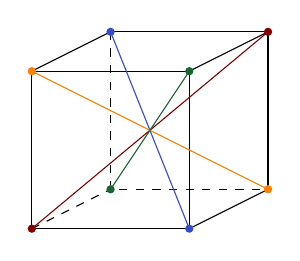
\begin{tikzpicture}
      \draw (0, 0) rectangle (2, 2);
      \draw (2, 0) -- +(1, 0.5);
      \draw (2, 2) -- +(1, 0.5);
      \draw (0, 2) -- +(1, 0.5);
      \draw [dashed] (0, 0) -- +(1, 0.5);
      \draw (1, 2.5) -- (3, 2.5) -- (3, 0.5);
      \draw [dashed] (1, 2.5) -- (1, 0.5) -- (3, 0.5);

      \draw [mred] (0, 0) node [circ] {} -- (3, 2.5) node [circ] {};
      \draw [mblue] (2, 0) node [circ] {} -- (1, 2.5) node [circ] {};
      \draw [morange] (0, 2) node [circ] {} -- (3, 0.5) node [circ] {};
      \draw [mgreen] (2, 2) node [circ] {} -- (1, 0.5) node [circ] {};
    \end{tikzpicture}
  \end{center}
  Then $G$ acts on $X$, and so we get $\phi: G \to \Sym(X)$. What is its kernel? To preserve the diagonals, it either does nothing, or flips the diagonals. So $G_X = \ker(\phi) = \{\id, \text{symmetry that sends each vertex to its opposite}\} \cong C_2$.

  How about the image? We have $G^X = \Im(\phi) \leq \Sym(X) \cong S_4$. It is an exercise to show that $\im(\phi) = \Sym(X)$, ie. it is surjective. We are not proving this because this is an exercise in geometry, not group theory. Then the first isomorphism theorem tells us
  \[
    G^X \cong G/G_X.
  \]
  So
  \[
    |G| = |G^X| |G_X| = 4! \cdot 2 = 48.
  \]
\end{eg}
This is an example of how we can use group actions to count elements in a group.

\begin{eg}[Cayley's theorem]
  For any group $G$, we have an action of $G$ on $G$ itself via
  \[
    g * g_1 = gg_1.
  \]
  It is trivial to check this is indeed an action. This gives a group homomorphism $\phi: G \to \Sym(G)$. What is its kernel? If $g \in \ker(\phi)$, then it acts trivially on every element. In particular, it acts trivially on the identity. So $g* e = e$, which means $g = e$. So $\ker(\phi) = \{e\}$. By the first isomorphism theorem, we get
  \[
    G \cong G/\{e\} \cong \im \phi \leq \Sym(G).
  \]
  So we know every group is (isomorphic to) a subgroup of a symmetric group.
\end{eg}

\begin{eg}
  Let $H$ be a subgroup of $G$, and $X = G/H$ be the set of left cosets of $H$. We let $G$ act on $X$ via
  \[
    g* g_1 H = gg_1 H.
  \]
  It is easy to check this is well-defined and is indeed a group action. So we get $\phi: G \to \Sym(X)$.

  Now consider $G_X = \ker(\phi)$. If $g \in G_X$, then for every $g_1 \in G$, we have $g * g_1 H = g_1H$. This means $g_1^{-1} gg_1 \in H$. In other words, we have
  \[
    g \in g_1 H g_1^{-1}.
  \]
  This has to happen for \emph{all} $g_1 \in G$. So
  \[
    G_X \subseteq \bigcap_{g_1 \in G} g_1 Hg_1^{-1}.
  \]
  This argument is completely reversible --- if $g \in \bigcap_{g_1 \in G} g_1 Hg_1^{-1}$, then
  \[
    g_1^{-1}g g_1 \in H,
  \]
  and hence
  \[
    gg_1 H = g_1H.
  \]
  So
  \[
    g* g_1 H = g_1 H
  \]
  for all $g_1 \in G$. So $g \in G_X$. Hence we indeed have equality:
  \[
    \ker (\phi) = G_X = \bigcap_{g_1 \in G} g_1 Hg_1^{-1}.
  \]
  Since this is a kernel, this is a normal subgroup of $G$, and is contained in $H$. Starting with an arbitrary subgroup $H$, this allows us to generate a normal subgroup, and this is indeed the biggest normal subgroup of $G$ that is in $H$, if we stare at it long enough.
\end{eg}

We can use this to prove the following theorem.
\begin{thm}
  Let $G$ be a finite group, and $H \leq G$ a subgroup of index $n$. Then there is a normal subgroup $K \lhd G$ with $K \leq H$ such that $G/K$ is isomorphic to a subgroup of $S_n$. Hence $|G/K| \mid n!$ and $|G/K| \geq n$.
\end{thm}

\begin{proof}
  We apply the previous example, giving $\phi: G \to \Sym(G/H)$, and let $K$ be the kernel of this homomorphism. We have already shown that $K \leq H$. Then the first isomorphism theorem gives
  \[
    G/K \cong \im \phi \leq \Sym(G/H) \cong S_n.
  \]
  The rest follows by Lagrange's theorem.
\end{proof}

\begin{cor}
  Let $G$ be a non-abelian simple group. Let $H \leq G$ be a proper subgroup of index $n$. Then $G$ is isomorphic to a subgroup of $A_n$. Moreover, we must have $n \geq 5$, ie. $G$ cannot have a subgroup of index less than $5$.
\end{cor}

\begin{proof}
  The action of $G$ on $X = G/H$ gives a homomorphism $\phi: G \to \Sym(X)$. Then $\ker(\phi) \lhd G$. Since $G$ is simple, $\ker(\phi)$ is either $G$ or $\{e\}$. We first show that it cannot be $G$. If $\ker(\phi) = G$, then every element of $G$ acts trivially on $X = G/H$. But if $g \in G\setminus H$, which exists since the index of $H$ is not $1$, then $g * H = gH \not= H$. So $g$ does not act trivially. So the kernel cannot be the whole of $G$. Hence $\ker(\phi) = \{e\}$.

  Thus by the first isomorphism theorem, we get
  \[
    G \cong \im (\phi) \leq \Sym(X) \cong S_n.
  \]
  We now need to show that $G$ is in fact a subgroup of $A_n$.

  Now $A_n \lhd S_n$. So $\im(\phi) \cap A_n \lhd \im(\phi) \cong G$. As $G$ is simple, $\im (\phi) \cap A_n$ is either $\{e\}$ or $G = \im(\phi)$. We want to show that the second thing happens, ie. the intersection is not the trivial group. We use the second isomorphism theorem. If $\im(\phi) \cap A_n = \{e\}$, then
  \[
    \im(\phi) \cong \frac{\im(\phi)}{\im(\phi) \cap A_n} \cong \frac{\im (\phi) A_n}{A_n} \leq \frac{S_n}{A_n} \cong C_2.
  \]
  So $G \cong \im (\phi)$ is a subgroup of $C_2$, ie. either $\{e\}$ or $C_2$ itself. Neither of these are non-abelian. So this cannot be the case. So we must have $\im(\phi) \cap A_n = \im(\phi)$, ie. $\im (\phi) \leq A_n$.

  The last part follows from the fact that $S_1, S_2, S_3, S_4$ have no non-abelian simple subgroups, which you can check by going to a quiet room and listing out all their subgroups.
\end{proof}

Let's recall some old definitions from IA Groups.
\begin{defi}[Orbit]
  If $G$ acts on a set $X$, the \emph{orbit} of $x \in X$ is
  \[
    G\cdot x = \{g * x \in X: g \in G\}.
  \]
\end{defi}

\begin{defi}[Stabilizer]
  If $G$ acts on a set $X$, the \emph{stabilizer} of $x \in X$ is
  \[
    G_x = \{g \in G: g * x = x\}.
  \]
\end{defi}

The main theorem about these concepts is the orbit-stabilizer theorem.
\begin{thm}[Orbit-stabilizer theorem]
  Let $G$ act on $X$. Then for any $x \in X$, there is a bijection between $G\cdot x$ and $G/G_x$, given by $g \cdot x \leftrightarrow g\cdot G_x$.

  In particular, if $G$ is finite, it follows that
  \[
    |G| = |G_x| |G \cdot X|.
  \]
\end{thm}
It takes some work to show this is well-defined and a bijection, but you've done it in IA Groups. In IA Groups, you probably learnt the second statement instead, but this result is more generally true for infinite groups.

\subsection{Conjugacy, centralizers and normalizers}
We have seen that every group acts on itself by multiplying on the left. A group $G$ can also act on itself in a different way, by conjugation:
\[
  g * g_1 = g g_1 g^{-1}.
\]
Let $\phi: G \to \Sym(G)$ be the associated permutation representation. Then
\[
  \phi(g) (g_1 \cdot g_2) = g g_1 g_2 g^{-1} = (g g_1 g^{-1})(g g_2 g^{-1}) = \phi(g)(g_1) \phi(g) (g_2).
\]
Thus we have shown that for each $g$, $\phi(g)$ is not just a map from $G$ to $G$, but a \emph{homomorphism} from $G$ to $G$. Since $\phi(g)$ is bijective (as in \emph{any} group action), it is in fact an isomorphism.

Thus, for any group $G$, there are many isomorphisms from $G$ to itself, one for every $g \in G$, and can be obtained from a group action of $G$ on itself.

Recall that at the beginning, we said groups are usually symmetries of some objects. Let's take a step further, and look at all symmetries of a group.
\begin{defi}[Automorphism group]
  The \emph{automorphism group} of $G$ is
  \[
    \Aut(G) = \{f: G \to G: f\text{ is a group isomorphism}\}.
  \]
  This is a group under composition, with the identity map as the identity.
\end{defi}
This is a subgroup of $\Sym(G)$, and the homomorphism $\phi: G\to \Sym(G)$ by conjugation lands in $\Aut(G)$.

This is pretty fun --- we can use this to cook up some more groups, by taking a group and looking at its automorphism group.

We can also take a group, take its automorphism group, and then take its automorphism group again, and do it again, and see if this process stabilizes, or becomes periodic.

\begin{defi}[Conjugacy class]
  The \emph{conjugacy class} of $g \in G$ is
  \[
    \ccl_G(g) = \{hgh^{-1}: h \in G\},
  \]
  ie. the orbit of $g \in G$ under the conjugation action.
\end{defi}

\begin{defi}[Centralizer]
  The \emph{centralizer} of $g \in G$ is
  \[
    C_G(g) = \{h \in G: hgh^{-1} = g\},
  \]
  ie. the stabilizer of $g$ under the conjugation action.
\end{defi}
This is alternatively the set of all $h \in G$ that commutes with $g$.

\begin{defi}[Center]
  The \emph{center} of a group $G$ is
  \[
    Z(G) = \{h \in G: hg h^{-1} = g\text{ for all }g \in G\} = \bigcap_{g \in G} C_G(g) = \ker (\phi).
  \]
\end{defi}
These are the elements of the group that commute with everything else.

By the orbit-stabilizer theorem, for each $x \in G$, we obtain a bijection $\ccl(x) \leftrightarrow G/C_G(x)$.
\begin{prop}
  Let $G$ be a finite group. Then
  \[
    |\ccl(x)| = |G:C_G(x)| = |G|/|C_G(x)|.
  \]
\end{prop}
In particular, the size of the conjugacy class divides the order of the group.

\begin{defi}[Normalizer]
  Let $H \leq G$. The \emph{normalizer} of $H$ in $G$ is
  \[
    N_G(H) = \{g \in G: g^{-1}H g = H\}.
  \]
\end{defi}
Note that we certainly have $H \leq N_G(H)$. Even better, $H \lhd N_G(H)$, essentially by definition. This is in fact the biggest subgroup of $G$ in which $H$ is normal.

We are now going to look at conjugacy classes of $S_n$. Now we recall from IA Groups that permutations in $S_n$ are conjugate if and only if they have the same cycle type when written as a product of disjoint cycles. We can think of the cycle types as partitions of $n$. For example, the partition $2, 2, 1$ of $5$ corresponds to the conjugacy class of $(1\; 2)(3\; 4)(5)$.

We will use this fact in the proof of the following theorem:
\begin{thm}
  The alternating groups $A_n$ are simple for $n \geq 5$ (also for $n = 1, 2, 3$).
\end{thm}
The cases in brackets follow from a direct check since $A_1 \cong A_2 \cong \{e\}$ and $A_3 \cong C_3$, all of which are simple. We can also check manually that $A_4$ has non-trivial normal subgroups, and hence not simple.

Recall we also proved that $A_5$ is simple in IA Groups by brute force --- we listed all its conjugacy classes, and see they cannot be put together to make a normal subgroup. This obviously cannot be easily generalized to higher values of $n$. Hence we need to prove this with a different approach.

\begin{proof}
  We start with the following claim:
  \begin{claim}
    $A_n$ is generated by $3$-cycles.
  \end{claim}
  As any element of $A_n$ is a product of evenly-many transpositions, it suffices to show that every product of two transpositions is also a product of $3$-cycles.

  There are three possible cases: let $a, b, c, d$ be distinct. Then
  \begin{enumerate}
    \item $(a\; b)(a\; b) = e$.
    \item $(a\; b)(b\; c) = (a\; b\; c)$.
    \item $(a\; b)(c\; d) = (a\; c\; b)(a\; c\; d)$.
  \end{enumerate}
  So we have shown that every possible product of two transpositions is a product of three-cycles.

  \begin{claim}
    Let $H \lhd A_n$. If $H$ contains a $3$-cycle, then we $H = A_n$.
  \end{claim}
  We show that if $H$ contains a $3$-cycle, then \emph{every} $3$-cycle is in $H$. Then we are done since $A_n$ is generated by $3$-cycles. For concreteness, suppose we know $(a\; b\; c) \in H$, and we want to show $(1\; 2\; 3) \in H$.

  Since they have the same cycle type, so we have $\sigma \in S_n$ such that $(a\; b\; c) = \sigma(1\; 2\; 3) \sigma^{-1}$. If $\sigma$ is even, ie. $\sigma \in A_n$, then we have that $(1\; 2\; 3) \in \sigma^{-1}H\sigma = H$, by the normality of $H$ and we are trivially done.

  If $\sigma$ is odd, replace it by $\bar{\sigma} = \sigma \cdot (4\; 5)$. Here is where we use the fact that $n \geq 5$ (we will use it again later). Then we have
  \[
    \bar{\sigma} (1\; 2\; 3) \bar{\sigma}^{-1} = \sigma (4\; 5)(1\; 2\; 3)(4\; 5) \sigma^{-1} = \sigma(1\; 2\; 3) \sigma^{-1} = (a\; b\; c),
  \]
  using the fact that $(1\; 2\; 3)$ and $(4\; 5)$ commute. Now $\bar{\sigma}$ is even. So $(1\; 2\; 3) \in H$ as above.

  What we've got so far is that if $H \lhd A_n$ contains \emph{any} $3$-cycle, then it is $A_n$. Finally, we have to show that every normal subgroup must contain at least one $3$-cycle.
  \begin{claim}
    Let $H \lhd A_n$ be non-trivial. Then $H$ contains a $3$-cycle.
  \end{claim}
  We separate this into many cases
  \begin{enumerate}
    \item Suppose $H$ contains an element which can be written in disjoint cycle notation
      \[
        \sigma = (1\; 2\; 3 \cdots r) \tau,
      \]
      for $r \geq 4$. We now let $\delta = (1\; 2\; 3) \in A_n$. Then by normality of $H$, we know $\delta^{-1} \sigma \delta \in H$. Then $\sigma^{-1}\delta^{-1}\sigma \delta \in H$. Also, we notice that $\tau$ does not contain $1, 2, 3$. So it commutes with $\delta$, and also trivially with $(1\; 2\; 3\; \cdots\; r)$. We can expand this mess to obtain
      \[
        \sigma^{-1} \delta^{-1} \sigma\delta = (r\; \cdots \; 2\; 1)(1\; 3\; 2)(1\; 2\; 3\; \cdots \; r)(1\; 2\; 3) = (2\; 3 \; r),
      \]
      which is a $3$-cycle. So done.

      The same argument goes through if $\sigma = (a_1 \; a_2 \; \cdots \; a_r) \tau$ for any $a_1, \cdots, a_n$.
    \item Suppose $H$ contains an element consisting of at least two $3$-cycles in disjoint cycle notation, say
      \[
        \sigma = (1\; 2\; 3)(4\; 5\; 6)\tau
      \]
      We now let $\delta = (1\; 2\; 4)$, and again calculate
      \[
        \sigma^{-1} \delta^{-1}\sigma\delta = (1\; 3\; 2)(4\; 6\; 5)(1\; 4\; 2)(1\; 2\; 3)(4\; 5\; 6)(1\; 2\; 4) = (1\; 2\; 4\; 3\; 6).
      \]
      This is a $5$-cycle, which is necessarily in $H$. By the previous case, we get a $3$-cycle in $H$ too, and hence $H = A_n$.
    \item Suppose $H$ contains $\sigma = (1\; 2\; 3)\tau$, with $\tau$ a product of $2$-cycles (if $\tau$ contains anything longer, then it would fit in one of the previous two cases). Then $\sigma^2 = (1\; 2\; 3)^2 = (1\; 3\; 2)$ is a three-cycle.
    \item Suppose $H$ contains $\sigma = (1\; 2)(3\; 4)\tau$, where $\tau$ is a product of $2$-cycles. We first let $\delta = (1\; 2\; 3)$ and calculate
      \[
        u = \sigma^{-1}\delta^{-1}\sigma\delta = (1\; 2)(3\; 4)(1\; 3\; 2)(1\; 2)(3\; 4)(1\; 2\; 3) = (1\; 4)(2\; 3),
      \]
      which is again in $u$. We landed in the same case, but instead of two transpositions times a mess, we just have two transpositions, which is nicer. Now let
      \[
        v = (1\; 5\; 2)u (1\; 2\; 5) = (1\; 3)(4\; 5) \in H.
      \]
      Note that we used $n \geq 5$ again. We have yet again landed in the same case. Notice however, that these are not the same transpositions. We multiply
      \[
        uv = (1\; 4)(2\; 3)(1\; 3)(4\; 5) = (1\; 2\; 3\; 4\; 5) \in H.
      \]
      This is then covered by the first case, and we are done.
  \end{enumerate}
  So done. Phew.
\end{proof}

\subsection{Finite $p$-groups}
Note that when studying the orders of groups and subgroups, we always talk about divisibility. We never talk about things like the sum of the orders to two subgroups. When it comes to divisibility, the simplest case would be when the order is a prime, and we have done that already. The next best thing we can hope for is that the order is a power of a prime.

\begin{defi}[$p$-group]
  A finite group $G$ is a \emph{$p$-group} if $|G| = p^n$ for some prime number $p$ and $n \geq 1$.
\end{defi}

\begin{thm}
  If $G$ is a finite $p$-group, then $Z(G) = \{x \in G: xg = gx\text{ for all }g \in G\}$ is non-trivial.
\end{thm}
This immediately tells us that for $n \geq 2$, a $p$ group is never simple.

\begin{proof}
  Let $G$ act on itself by conjugation. The orbits of this action (ie. the conjugacy classes) have order dividing $|G| = p^n$. So it is either a singleton, or its size is divisible by $p$.

  Since the conjugacy classes partition $G$, we know the total size of the conjugacy classes is $|G|$. In particular,
  \begin{multline*}
    |G| = \text{number of conjugacy class of size 1} \\
    + \sum \text{order of all other conjugacy classes}.
  \end{multline*}
  We know the second term is divisible by $p$. Also $|G| = p^n$ is divisible by $p$. Hence the number of conjugacy classes of size $1$ is divisible by $p$. We know $\{e\}$ is a conjugacy class of size $1$. So there must be at least $p$ conjugacy classes of size $1$. Since the smallest prime number is $2$, there is a conjugacy class $\{x\} \not= \{e\}$.

  But if $\{x\}$ is a conjugacy class on its own, then by definition $g^{-1}xg = x$ for all $g \in G$, ie. $xg = gx$ for all $g \in G$. So $x \in Z(G)$. So $Z(G)$ is non-trivial.
\end{proof}
The theorem allows us to prove interesting things about $p$-groups by induction --- we can quotient $G$ by $Z(G)$, and get a smaller $p$-group. One way to do this is via the below lemma.

\begin{lemma}
  For any group $G$, if $G/Z(G)$ is cyclic, then $G$ is abelian.

  In other words, if $G/Z(G)$ is cyclic, then it is in fact trivial, since the center of an abelian group is the abelian group itself.
\end{lemma}

\begin{proof}
  Let $gZ(G)$ be a generator of the cyclic group $G/Z(G)$. Hence every coset of $Z(G)$ is of the form $g^rZ(G)$. So every element $x \in G$ must be of the form $g^r z$ for $z \in Z(G)$ and $r \in \Z$. To show $G$ is abelian, let $\bar{x} = g^{\bar{r}} \bar{z}$ be another element, with $\bar{z} \in Z(G), \bar{r} \in \Z$. Note that $z$ and $\bar{z}$ are in the center, and hence commute with every element. So we have
  \[
    x\bar{x} = g^r z g^{\bar{r}} \bar{z} = g^r g^{\bar{r}} z \bar{z} = g^{\bar{r}}g^r \bar{z} z = g^{\bar{r}}\bar{z} g^r z = \bar{x} x.
  \]
  So they commute. So $G$ is abelian.
\end{proof}

This is a general lemma for groups, but is particularly useful when applied to $p$ groups.
\begin{cor}
  If $p$ is prime and $|G| = p^2$, then $G$ is abelian.
\end{cor}

\begin{proof}
  Since $Z(G) \leq G$, its order must be $1$, $p$ or $p^2$. Since it is not trivial, it can only be $p$ or $p^2$. If it has order $p^2$, then it is the whole group and the group is abelian. Otherwise, $G/Z(G)$ has order $p^2/p = p$. But then it must be cyclic, and thus $G$ must be abelian. This is a contradiction. So $G$ is abelian.
\end{proof}

\begin{thm}
  Let $G$ be a group of order $p^a$, where $p$ is a prime number. Then it has a subgroup of order $p^b$ for any $0 \leq b \leq a$.
\end{thm}
This means there is a subgroup of every conceivable order. This is not true for general groups. For example, $A_5$ has no subgroup of order $30$ or else that would be a normal subgroup.

\begin{proof}
  We induct on $a$. If $a = 1$, then $\{e\}, G$ give subgroups of order $p^0$ and $p^1$. So done.

  Now suppose $a > 1$, and we want to construct a subgroup of order $p^b$. If $b = 0$, then this is trivial, namely $\{e\} \leq G$ has order $1$.

  Otherwise, we know $Z(G)$ is non-trivial. So let $x \not= e \in Z(G)$. Since $x \mid |G|$, its order is a power of $p$. If it in fact has order $p^c$, then $x^{p^{c - 1}}$ has order $p$. So we can suppose, by renaming, that $x$ is order $p$. We have thus generated a subgroup $\bra x\ket$ of order exactly $p$. Moreover, since $x$ is in the center, $\bra x\ket$ commutes with everything in $G$. So $\bra x\ket$ is in fact a normal subgroup of $G$. This is the point of choosing it in the center. Therefore $G/\bra x\ket$ has order $p^{a - 1}$.

  Since this is a strictly smaller group, we can by induction suppose $G/\bra x\ket$ has a subgroup of any order. In particular, it has a subgroup $L$ of order $p^{b - 1}$. By the subgroup correspondence, there is some $K \leq G$ such that $L = K / \bra x\ket$ and $H \lhd K$. But then $K$ has order $p^b$. So done.
\end{proof}

\subsection{Finite abelian groups}
We now move on to a small section, which is small because we will come back to it later.

It turns out finite abelian groups are very easy to classify. We can just write down a list of all finite abelian groups. We write down the classification theorem, and then prove it in the last part of the course.

\begin{thm}[Classification of finite abelian groups]
  Let $G$ be a finite abelian group. Then there exists some $d_1, \cdots, d_r$ such that
  \[
    G \cong C_{d_1} \times C_{d_2} \times \cdots \times C_{d_r}.
  \]
  Moreover, we can pick $d_i$ such that $d_{i + 1} \mid d_i$ for each $i$, and this expression is unique.
\end{thm}
It turns out the best way to prove this is not to think of it as a group, but as a $\Z$-module, which is something we will come to later.

\begin{eg}
  The abelian groups of order $8$ are $C_8$, $C_4 \times C_2$, $C_2 \times C_2 \times C_2$.
\end{eg}

\begin{lemma}
  If $n$ and $m$ are coprime, then $C_{mn} \cong C_m \times C_n$.
\end{lemma}
This is a grown-up version of the Chinese remainder theorem. This is what the Chinese remainder theorem really says.

\begin{proof}
  It suffices to find an element of order $nm$ in $C_m \times C_n$. Then since $C_n \times C_m$ has order $nm$, it must be cyclic, and hence isomorphic to $C_{nm}$.

  Let $g \in C_m$ have order $m$; $h \in C_n$ have order $n$, and consider $(g, h) \in C_m \times C_n$. Suppose the order of $(g, h)$ is $k$. Then $(g, h)^k = (e, e)$. Hence $(g^k, h^k) = (e, e)$. So the order of $g$ and $h$ divide $k$, ie. $m \mid k$ and $n \mid k$. As $m$ and $n$ are coprime, this means that $mn \mid k$.

  As $k = \ord((g, h))$ and $(g, h) \in C_m \times C_n$ is a group of order $mn$, we must have $k \mid nm$. So $k = nm$.
\end{proof}

\begin{cor}
  For any finite abelian group $G$, we have
  \[
    G \cong C_{d_1} \times C_{d_2} \times \cdots \times C_{d_r},
  \]
  where each $d_i$ is some prime power.
\end{cor}

\begin{proof}
  From the classification theorem, iteratively apply the previous lemma to break each component up into products of prime powers.
\end{proof}

As promised, this is short.

\subsection{Sylow theorems}
\begin{thm}[Sylow theorems]
  Let $G$ be a finite group of order $p^a \cdot m$, with $p$ and prime and $p \nmid m$. Then
  \begin{enumerate}
    \item The set of Sylow $p$-subgroups of $G$, given by
      \[
        \Syl_p(G) = \{P \leq G: |P| = p^a\},
      \]
      is non-empty. In other words, $G$ has a subgroup of of order $p^a$.
    \item All elements of $\Syl_p(G)$ are conjugate in $G$.
    \item The number of Sylow $p$-subgroups $n_p = |\Syl_p(G)|$ satisfies $n_p \equiv 1 \pmod p$ and $n_p \mid |G|$ (in fact $n_p \mid m$, since $p$ is not a factor of $n_p$).
  \end{enumerate}
\end{thm}
These are sometimes known as Sylow's first/second/third theorem respectively.

We will not prove this just yet. We first look at how we can apply this theorem. We can use it without knowing how to prove it.

\begin{lemma}
  If $n_p = 1$, then the Sylow $p$-subgroups is normal in $G$.
\end{lemma}

\begin{proof}
  Let $P$ be the unique Sylow $p$-subgroup, and let $g \in G$, and consider $g^{-1}Pg$. Since this is isomorphic to $p$, we must have $|g^{-1} Pg| = p^a$, ie. it is also a Sylow $p$-subgroup. Since there is only one, we must have $P = g^{-1}Pg$. So $P$ is normal.
\end{proof}

\begin{cor}
  Let $G$ be a non-abelian simple group. Then $|G| \mid \frac{n_p!}{2}$ for every prime $p$ such that $p \mid |G|$.
\end{cor}

\begin{proof}
  The group $G$ acts on $\Syl_p(G)$ by conjugation. So it gives a permutation representation $\phi: G \to \Sym(\Syl_p(G)) \cong S_{n_p}$. We know $\ker \phi \lhd G$. But $G$ is simple. So $\ker(\phi)= \{e\}$ or $G$. We want to show it is not the whole of $G$.

  If we had $G = \ker(\phi)$, then $g^{-1} Pg = P$ for all $g \in G$. Hence $P$ is a normal subgroup. As $G$ is simple, either $P = \{e\}$, or $P = G$. We know $P$ cannot be trivial since $p \mid |G|$. But if $G = P$, then $G$ is a $p$-group, has a non-trivial center, and hence $G$ is not non-abelian simple. So we must have $\ker(\phi) = \{e\}$.

  Then by the first isomorphism, we know $G \cong \im \phi \leq S_{n_p}$. We have proved the theorem without the divide-by-two part. To prove the whole result, we need to show that in fact $\im (\phi) \leq A_{n_p}$. Consider the following composition of homomorphisms:
  \[
    \begin{tikzcd}
      G \ar[r, "\phi"] & S_{n_p} \ar[r, "\sgn"] & \{\pm 1\}.
    \end{tikzcd}
  \]
  If this is surjective, then $\ker (\sgn \circ \phi) \lhd G$ has index $2$ (since the index is the size of the image), and is not the whole of $G$. This means $G$ is not simple (the case where $|G| = C_2$ is ruled out since it is non-abelian).

  So the kernel must be the whole $G$, and $\sgn \circ \phi$ is the trivial map. In other words, $\sgn(\phi(g)) = +1$. So $\phi(g) \in A_{n_p}$. So in fact we have
  \[
    G \cong \im(\phi) \leq A_{n_p}.
  \]
  So we get $|G| \mid \frac{n_p!}{2}$.
\end{proof}

\begin{eg}
  Suppose $|G| = 1000$. Then $|G|$ is not simple. To show this, we need to factorize $1000$. We have $|G| = 2^3 \cdot 5^3$. We pick our favorite prime to be $p = 5$. We know $n_5 \cong 1 \pmod 5$, and $n_5 \mid 2^3 = 8$. The only number that satisfies this is $n_5 = 1$. So the Sylow $5$-subgroup is normal, and hence $G$ is not normal.
\end{eg}

\begin{eg}
  Let $|G| = 132 = 2^2 \cdot 3 \cdot 11$. We want to show this is not simple. So for a contradiction suppose it is.

  We start by looking at $p = 11$. We know $n_{11} \equiv 1 \pmod {11}$. Also $n_{11} \mid 12$. As $G$ is simple, we must have $n_{11} = 12$.

  Now look at $p = 3$. We have $n_3 = 1 \pmod 3$ and $n_3 \mid 44$. The possible values of $n_3$ are $4$ and $22$.

  If $n_3 = 4$, then the corollary says $|G| \mid \frac{4!}{2} = 12$, which is of course nonsense. So $n_3 = 22$.

  At this point, we count how many elements of each order there are. This is particularly useful if $p \mid |G|$ but $p^2 \nmid |G|$, ie. the Sylow $p$-subgroups have order $p$ and hence are cyclic.

  As all Sylow $11$-subgroups are disjoint, apart from $\{e\}$, we know there are $12 \cdot (11 - 1) = 120$ elements of order $11$. We do the same thing with the Sylow $3$-subgroups. We need $22 \cdot (3 - 1) = 44$ elements of order $3$. But this is more elements than the group has. This can't happen. So $G$ must be simple.
\end{eg}

\begin{proof}(of Sylow's theorem)
  Let $G$ be a finite group with $|G| = p^a m$, and $p \nmid m$.
  \begin{enumerate}
    \item We need to show that $\Syl_p(G) \not= \emptyset$, ie. we need to find some subgroup of order $p^a$. As always, we find something clever for $G$ to act on. We let
      \[
        \Omega = \{X\text{ sub\emph{set} of }G: |X| = p^a\}.
      \]
      We let $G$ act on $\Omega$ by
      \[
        g * \{g_1, g_2, \cdots, g_{p^a}\} = \{gg_1, gg_2, \cdots, gg_{p^a}\}.
      \]
      Let $\Sigma \leq \Omega$ be an orbit.

      We first note that if $\{g_1, \cdots, g_{p^1}\} \in \Sigma$, then by the definition of an orbit, for every $g \in G$,
      \[
        gg_1^{-1} * \{g_1, \cdots, g_{p^a}\} = \{g, gg_1^{-1}g_2, \cdots, gg_1^{-1} g_{p^a}\} \in \Sigma.
      \]
      The important thing is that this set contains $g$. So for each $g$, $\Sigma$ contains a set $X$ which contains $g$. Since each set $X$ has size $p^a$, we must have
      \[
        |\Sigma| \geq \frac{|G|}{p^a} = m.
      \]
      Suppose $|\Sigma| = m$. Then the orbit-stabilizer theorem says the stabilizer $H$ of any $\{g_1, \cdots, g_{p^a}\} \in \Sigma$ has index $m$, hence $|H| = p^a$, and thus $H \in \Syl_p(G)$.

      So we need to show that not every orbit $\Sigma$ can have size $> m$. Again, by the orbit-stabilizer, the size of any orbit divides the order of the group, $|G| = p^a m$. So if $|\Sigma| > m$, then $p \mid |\Sigma|$. Suppose we can show that $p \nmid |\Omega|$. Then not every orbit $\Sigma$ can have size $> m$, since $\Omega$ is the disjoint union of all the orbits, and thus we are done.

      So it suffices to show $p \nmid |\Omega|$. We can count
      \[
        |\Omega| = \binom{|G|}{p^a} = \binom{p^a m}{p^a} = \prod_{j = 0}^{p^a - 1} = \frac{p^a m - j}{p^a - j}.
      \]
      Now note that the largest power of $p$ dividing $p^am - j$ is the largest power of $p$ dividing $j$. Similarly, the largest power of $p$ dividing $p^a - j$ is also the largest power of $p$ dividing $j$. So we have the same power of $p$ on top and bottom for each item in the product, and they cancel. So the result is not divisible by $p$.

      This proof is not straightforward. We first needed the clever idea of letting $G$ act on $\Omega$. But then if we are given this set, the obvious thing to do would be to find something in $\Omega$ that is also a group. This is not what we do. Instead, we find an orbit whose stabilizer is a Sylow $p$-subgroup.
    \item We instead prove something stronger: if $Q \leq G$ is a $p$-subgroup (ie. $|Q| = p^b$, for $b$ not necessarily $a$), and $P \leq G$ be a Sylow $p$-subgroup, then there is a $g \in G$ such that $g^{-1} Qg \leq P$. Applying this to the case where $Q$ is another Sylow $p$-subgroup says there is a $g$ such that $g^{-1}Qg \leq P$, but since $g^{-1}Qg$ has the same size as $P$, they must be equal.

      We let $Q$ act on the set of cosets of $G/P$ via
      \[
        q * gP = qgP.
      \]
      We know the orbits of this action have size dividing $|Q|$, so is either $1$ or divisible by $p$. But they can't all be divisible by $p$, since $|G/P|$ is coprime to $p$. So at least one of them have size $1$, say $\{gP\}$. In other words, for every $q \in Q$, we have $qgP = gP$. This means $g^{-1}qg \in P$. This holds for every element $q \in Q$. So we have found a $g$ such that $g^{-1}Qg \leq P$.

    \item Finally, we need to show that $n_p \cong 1 \pmod p$ and $n_p \mid |G|$, where $n_p = |\Syl_P(G)|$.

      The second part is easier --- by Sylow's second theorem, the action of $G$ on $\Syl_p(G)$ by conjugation has one orbit. By the orbit-stabilizer theorem, the size of the orbit, which is $|\Syl_p(G)| = n_p$, divides $|G|$. This proves the second part.

      For the first part, let $P \in \Syl_P(G)$. Consider the action by conjugation of $P$ on $\Syl_p(G)$. Again by the orbit-stabilizer theorem, the orbits each have size $1$ or size divisible by $p$. But we know there is one orbit of size $1$, namely $\{P\}$ itself. To show $n_p = |\Syl_P(G)| \cong 1\pmod p$, it is enough to show there are no other orbits of size $1$.

      Suppose $\{Q\}$ is an orbit of size $1$. This means for every $p \in P$, we get
      \[
        p^{-1} Qp = Q.
      \]
      In other words, $P \leq N_G(Q)$. Now $N_G(Q)$ is itself a group, and we can look at its Sylow $p$-subgroups. We know $Q \leq N_G(Q) \leq G$. So $p^a \mid |N_G(Q)| \mid p^a m$. So $p^a$ is the biggest power of $p$ that divides $|N_G(Q)|$. So $Q$ is a Sylow $p$-subgroup of $N_G(Q)$.

      Now we know $P \leq N_G(Q)$ is \emph{also} a Sylow $p$-subgroup of $N_G(Q)$. By Sylow's second theorem, they must be conjugate in $N_G(Q)$. But conjugating anything in $Q$ by something in $N_G(Q)$ does nothing, by definition of $N_G(Q)$. So we must have $P = Q$. So the only orbit of size $1$ is $\{P\}$ itself. So done.
  \end{enumerate}
\end{proof}

This is all the theories of groups we've got. In the remaining time, we will look at some interesting examples of groups.
\begin{eg}
  Let $G = \GL_n(\Z/p)$, ie. the set of invertible $n\times n$ matrices with entries in $\Z/p$, the integers modulo $p$. Here $p$ is obviously a prime. When we do rings later, we will study this properly.

  First of all, we would like to know the size of this group. A matrix $A \in \GL_n(\Z/p)$ is the same as $n$ linearly independent vectors in the vector space $(\Z/p)^n$. We can just work out how many there are. This is not too difficult, when you know how.

  We can pick the first vector, which can be anything except zero. So there are $p^n - 1$ ways of choosing the first vector. Next, we need to pick the second vector. This can be anything that is not in the span of the first vector, and this rules out $p$ possibilities. So there are $p^n - p$ ways of choosing the second vector. Continuing this chain of thought, we have
  \[
    |\GL_n(\Z/p)| = (p^n - 1)(p^n - p)(p^n - p^2) \cdots (p^n - p^{n - 1}).
  \]
  What is a Sylow $p$-subgroup of $\GL_n(\Z/p)$? We first work out what the order of this is. We can factorize that as
  \[
    |\GL_n(\Z/p)|= (1 \cdot p \cdot p^2 \cdot \cdots \cdot p^{n - 1}) ((p^n - 1)(p^{n - 1} - 1) \cdots (p - 1)).
  \]
  So the largest power of $p$ that divides $|\GL_n(\Z/p)|$ is $p^{\binom{n}{2}}$. Let's find a subgroup of size $p^{\binom{n}{2}}$. We consider matrices of the form
  \[
    U = \left\{
      \begin{pmatrix}
        1 & * & * & \cdots & *\\
        0 & 1 & * & \cdots & *\\
        0 & 0 & 1 & \cdots & *\\
        \vdots & \vdots & \vdots & \ddots & \vdots\\
        0 & 0 & 0 & \cdots & 1
      \end{pmatrix} \in \GL_n(\Z/p)
    \right\}.
  \]
  Then we know $|U| = p^{\binom{n}{2}}$ as each $*$ can be chosen to be anything in $\Z/p$, and there are $\binom{n}{2}$ $*$s.

  Is the Sylow $p$-subgroup unique? No. We can take the lower triangular matrices and get another Sylow $p$-subgroup.
\end{eg}

\begin{eg}
  Let's be less ambitious and consider $\GL_2(\Z/p)$. So
  \[
    |G| = p(p^2 - 1)(p - 1) = p(p - 1)^2 (p + 1).
  \]
  Let $\ell$ be another prime number such that $\ell \mid p - 1$. Suppose the largest power of $\ell$ that divides $|G|$ is $\ell^2$. Can we (explicitly) find a Sylow $\ell$-subgroup?

  First, we want to find an element of order $\ell$. How is $p - 1$ related to $p$ (apart from the obvious way)? We know that
  \[
    (\Z/p)^\times = \{x \in \Z/p:(\exists y)\, xy \equiv 1 \pmod p\} \cong C_{p - 1}.
  \]
  So as $\ell\mid p - 1$, there is a subgroup $C_\ell \leq C_{p - 1} \cong (\Z/p)^\times$. Then we immediately know where to find a subgroup of order $\ell^2$: we have
  \[
    C_\ell \times \C_\ell \leq (\Z/p)^* \times (\Z/p)^\times \leq \GL_2(\Z/p),
  \]
  where the final inclusion is the diagonal matrices, identifying
  \[
    (a, b) \leftrightarrow
    \begin{pmatrix}
      a & 0\\
      0 & b
    \end{pmatrix}.
  \]
  So this is the Sylow $\ell$-subgroup.
\end{eg}

\section{Rings}
\subsection{Definitions and examples}
\begin{defi}[Ring]
  A \emph{ring} is a quintuple $(R, +, \ph, 0_R, 1_R)$ where $0_R, 1_R \in R$, and $+, \ph: R \times R \to R$ are binary operations such that
  \begin{enumerate}
    \item $(R, +, 0_R)$ is an abelian group.
    \item The operation $\ph: R \times R \to R$ satisfies associativity, ie.
      \[
        a\cdot (b\cdot c) = (a \cdot b)\cdot c,
      \]
      and identity:
      \[
        1_R \cdot r = r \cdot 1_R = r.
      \]
    \item Multiplication distributes over addition, ie.
      \begin{align*}
        r_1 \cdot (r_2 + r_3) &= (r_1 \cdot r_2) + (r_1 \cdot r_3)\\
        (r_1 + r_2) \cdot r_3 &= (r_1 \cdot r_3) + (r_2 \cdot r_3).
      \end{align*}
  \end{enumerate}
\end{defi}
Some people don't insist on the existence of the multiplicative identity, but we will assume they exist.

Since we can add and multiply two elements, by induction, we can add and multiply any finite number of elements. However, the notions of infinite sum and product are undefined. It doesn't make sense to ask if an infinite sum converges.

\begin{defi}[Commutative ring]
  We say a ring $R$ is \emph{commutative} if $a \cdot b = b \cdot a$ for all $a, b \in R$.
\end{defi}

From now onwards, all rings in this course are going to be commutative.

Just as we have groups and subgroups, we also have subrings.
\begin{defi}[Subring]
  Let $(R, +, \ph, 0_R, 1_R)$ be a ring, and $S \subseteq R$ is a subset. We say $S$ is a \emph{subring} of $R$ if $0_R, 1_R \in S$, and the operations $+, \ph$ make $S$ into a ring in its own right. In this case we write $S \leq R$.
\end{defi}

\begin{eg}
  The familiar number systems are all rings: we have $\Z \leq \Q \leq \R \leq \C$, under the usual $0, 1, +, \ph$.
\end{eg}

\begin{eg}
  The set $\Z[i] = \{a + ib: a, b \in \Z\} \leq \C$ is the \emph{Gaussian integers}, which is a ring.

  We also have the ring $\Q[\sqrt{2}] = \{a + b \sqrt{2} \in \R: a, b \in \Q\} \leq \R$.
\end{eg}
This notation with square brackets will become clear when we define them properly later.

\begin{defi}[Unit]
  An element $u \in R$ is a \emph{unit} if there is another element $v \in R$ such that $u \cdot v = 1_R$.
\end{defi}
In other words, units are the things that have inverses.

It is important that this depends on $R$, not just on $u$. For example, $2 \in \Z$ is not a unit, but $2 \in \Q$ is a unit (since $\frac{1}{2}$ is an inverse).

A very nice situation is when (almost) everything is a unit.
\begin{defi}[Field]
  A \emph{field} is a ring where every $u \not= 0_R \in R$ is a unit.
\end{defi}
We will later show that $0_R$ cannot be a unit unless in a very degenerate case.

\begin{eg}
  $\Z$ is not a field, but $\Q, \R, \C$ are all fields.

  Similarly, $\Z[i]$ is not a field, while $\Q[\sqrt{2}]$ is.
\end{eg}

\begin{notation}
  If $R$ is a ring and $r \in R$, we write $-r$ for the inverse to $r$ in $(R, +, 0_R)$. This satisfies $r + (-r) = 0_R$. We write $r - s$ to mean $r + (-s)$ etc.
\end{notation}

\begin{eg}
  Let $R$ be a ring. Then $0_R + 0_R = 0_R$, since this is true in the group $(R, +, 0_R)$. Then for any $r \in R$, we get
  \[
    r(0_R + 0_R) = r 0_R.
  \]
  We now use the fact that multiplication distributions over multiplication. So
  \[
    r \cdot 0_R + r \cdot 0_R = r \cdot 0_R.
  \]
  Adding $(-r \cdot 0_R)$ to both sides give
  \[
    r \cdot 0_R = 0_R.
  \]
  This is true for any element $r \in R$. In particular, if $R \not= \{0\}$, then $1_R \not= 0_R$. If they were equal, then take $r \not= 0_R$. So
  \[
    r = r \cdot 1_R = r \cdot 0_R = 0_R,
  \]
  which is a contradiction.
\end{eg}
Note, however, that $\{0\}$ forms a ring (with the only possible operations and identities), the zero ring, albeit a boring one. However, this is often a counterexample to many things.

\begin{defi}[Product of rings]
  Let $R, S$ be rings. Then the \emph{product} $R \times S$ is a ring via
  \[
    (r, s) + (r', s') = (r + r', s + s'),\quad (r, s) \cdot (r', s') = (r\cdot r', s \cdot s').
  \]
  The zero is $(0_R, 0_S)$ and the one is $(1_R, 1_S)$.

  We can (but won't) check that these indeed are rings.
\end{defi}

\begin{defi}[Polynomial]
  Let $R$ be a ring. Then a \emph{polynomial} with coefficients in $R$ is an expression
  \[
    f = a_0 + a_1X + a_2 X^2 + \cdots + a_n X^n,
  \]
  with $a_i \in R$. The symbols $X^i$ are formal symbols.
\end{defi}
We identify $f$ and $f + 0_R \cdot X^{n + 1}$ as the same things.

\begin{defi}[Degree of polynomial]
  The \emph{degree} of a polynomial $f$ is the largest $m$ such that $a_m \not= 0$.
\end{defi}

\begin{defi}[Monic polynomial]
  Let $f$ have degree $m$. If $a_m = 1$, then $f$ is called \emph{monic}.
\end{defi}

\begin{defi}[Polynomial ring]
  We write $R[X]$ for the set of all polynomials with coefficients in $R$. The operations are performed in the obvious way, ie. if $f = a_0 + a_1X + \cdots + A_n X$ and $g = b_0 + b_1X + \cdots + b_k X^k$ are polynomials, then
  \[
    f + g = \sum_{r = 0}^{\max\{n, k\}} (a_i + b_i) X^i,
  \]
  and
  \[
    f\cdot g = \sum_{i = 0}^{n + k} \left(\sum_{j = 0}^i a_j b_{i - j}\right) X^i,
  \]
  We identify $R$ with the constant polynomials, ie. polynomials $\sum a_i X^i$ with $a_i = 0$ for $i > 0$. In particular, $0_R \in R$ and $1_R \in R$ are the zero and one of $R[x]$.
\end{defi}
This is in fact a ring.

Note that a polynomial is just a sequence of numbers, interpreted as the coefficients of some formal symbols. While it does indeed induce a function in the obvious way, we shall not identify the polynomial with the function given by it, since different polynomials can give rise to the same function.

For example, in $\Z/2\Z [X]$, $f = X^2 + X$ is not the zero polynomial, since its coefficients are not zero. However, $f(0) = 0$ and $f(1) = 0$. As a function, this is identically zero. So $f \not= 0$ as a polynomial but $f = 0$ as a function.

\begin{defi}[Power series]
  We write $R[[x]]$ for the ring of power series on $R$, ie.
  \[
    f = a_0 + a_1 X + a_2 X^2 + \cdots,
  \]
  where each $a_i \in R$. This has addition and multiplication the same as for polynomials, but without upper limits.
\end{defi}
A power series is very not a function. We don't talk about whether the sum converges or not, because it is not a sum.

How are polynomials and power series different?

\begin{eg}
  Is $1 - X \in R[X]$ a unit? For every $g = a_0 + \cdots + a_n X^n$ (with $a_n \not= 0$), we get
  \[
    (1 - X)g = \text{stuff} + \cdots - a_n X^{n + 1},
  \]
  which is not $1$. So $g$ cannot be the inverse of $(1 - X)$.

  However, $1 - x \in R[[X]]$ \emph{is} a unit, since
  \[
    (1 - X)(1 + X + X^2 + X^3 + \cdots) = 1.
  \]
\end{eg}

\begin{defi}[Laurent polynomials]
  The \emph{Laurent polynomials} on $R$ is the set $R[X, X^{-1}]$, ie. each element is of the form
  \[
    f = \sum_{i \in \Z} a_i X^i
  \]
  where $a_i \in R$ and only finitely many $a_i$ are non-zero. The operations are the obvious ones.
\end{defi}
We can also think of Laurent series, but we have to be careful. We allow infinitely many positive coefficients, but only finitely many negative ones. Or else, in the formula for multiplication, we will have an infinite sum, which is undefined.

\begin{eg}
  Let $X$ be a set, and $R$ be a ring. Then the set of all functions on $X$, ie. functions $f: X \to R$ is a ring given by
  \[
    (f + g)(x) = f(x) + g(x),\quad (f\cdot g)(x) = f(x) \cdot g(x).
  \]
  Here zero is the constant function $0$ and one is the constant function $1$.

  Usually, we don't want to consider all functions $X \to R$. Instead, we look at some subrings of this. For example, we can consider the ring of all continuous functions $\R \to \R$. This contains, for example, the polynomial functions, which is just $\R[X]$ (since in $\R$, polynomials \emph{are} functions).
\end{eg}

\subsection{Homomorphisms, ideals, quotients and isomorphisms}
Just like groups, we will come up with analogues of homomorphisms, normal subgroups (which are now known as ideals), and quotient rings.

\begin{defi}[Homomorphism of rings]
  Let $R, S$ be rings. A function $\phi: R \to S$ is a \emph{ring homomorphism} if it preserves everything we can think of, ie.
  \begin{enumerate}
    \item $\phi(r_1 + r_2) = \phi(r_1) + \phi(r_2)$,
    \item $\phi(0_R) = 0_S$,
    \item $\phi(r_1 \cdot r_2) = \phi(r_1) \cdot \phi(r_2)$,
    \item $\phi(1_R) = 1_S$.
  \end{enumerate}
\end{defi}

\begin{defi}[Isomorphism of rings]
  If a homomorphism $\phi: R \to S$ is a bijection, we call it an \emph{isomorphism}.
\end{defi}

\begin{defi}[Kernel]
  The \emph{kernel} of a homomorphism $\phi: R \to S$ is
  \[
    \ker (\phi) = \{r \in R: \phi(r) = 0_S\}.
  \]
\end{defi}

\begin{defi}[Image]
  The \emph{image} of $\phi: R \to S$ is
  \[
    \im(\phi) = \{s \in S: s = \phi(r) \text{ for some }r \in R\}.
  \]
\end{defi}

\begin{lemma}
  A homomorphism $\phi: R \to S$ is injective if and only if $\ker \phi = \{0_R\}$.
\end{lemma}

\begin{proof}
  A ring homomorphism is in particular a group homomorphism $\phi: (R, +, 0_R) \to (S, +, 0_S)$ of abelian groups. So this follows from the case of groups.
\end{proof}

In the group scenario, we had groups, subgroups and \emph{normal} subgroups, which are special subgroups. Here, we have a special kind of subsets of a ring that act like normal subgroups, known as \emph{ideals}.

\begin{defi}[Ideal]
  A subset $I \subseteq R$ is an \emph{ideal}, written $I \lhd R$, if
  \begin{enumerate}
    \item It is an additive subgroup of $(R, +, 0_R)$, ie. it is closed under addition and additive inverses.\hfill (additive closure)
    \item If $a \in I$ and $b \in R$, then $a \cdot b \in I$. \hfill (strong closure)
  \end{enumerate}
  We say $I$ is a proper ideal if $I \not= R$.
\end{defi}
Note that the multiplicative closure is stronger than what we require for subrings --- for subrings, it has to be closed under multiplication by its own elements; for ideals, it has to be closed under multiplication by everything in the world. This is similar to how normal subgroups not only have to be closed under internal multiplication, but also conjugation by external elements.

\begin{lemma}
  If $\phi: R \to S$ is a homomorphism, then $\ker(\phi)\lhd R$.
\end{lemma}

\begin{proof}
  Since $\phi: (R, +, 0_R) \to (S, +, 0_R)$ is a group homomorphism, the kernel is a subgroup of $(R, +, 0_R)$.

  For the second part, let $a \in \ker(\phi)$, $b \in R$. We need to show that their product is in the kernel. We have
  \[
    \phi(a\cdot b) = \phi(a) \cdot \phi(b) = 0 \cdot \phi(b) = 0.
  \]
  So $a \cdot b \in \ker(\phi)$.
\end{proof}

\begin{eg}
  Suppose $I \lhd R$ is an ideal, and $1_R \in I$. Then for any $r \in R$, the axioms entail $1_R \cdot r \in I$. But $1_R \cdot r = r$. So if $1_R \in I$, then $I = R$.

  In other words, every proper ideal does not contain $1$. In particular, every proper ideal is not a subring, since a subring must contain $1$.
\end{eg}
We are starting to diverge from groups. In groups, a normal subgroup is a subgroup, but here an ideal is not a subring.

\begin{eg}
  We can generalize the above a bit. Suppose $I \lhd R$ and $u \in I$ is a unit, ie. there is some $v \in R$ such that $uv = 1_R$. Then by strong closure, $1_R = u \cdot v\in I$. So $I = R$.

  Hence proper ideals are not allowed to contain any unit at all, not just $1_R$.
\end{eg}

\begin{eg}
  Consider the ring $\Z$ of integers. Then every ideal of $\Z$ is of the form
  \[
    n\Z = \{\cdots, -2n, -n, 0, n, 2n, \cdots\} \subseteq \Z.
  \]
  It is easy to see this is indeed an ideal.

  To show these are all the ideals, let $I \lhd \Z$. If $I = \{0\}$, then $I = 0\Z$. Otherwise, let $n \in N$ be the smallest positive element of $T$. We want to show in fact $I = n\Z$. Certainly $n\Z \subseteq I$ by strong closure.

  Now let $m \in I$. By the Euclidean algorithm, we can write
  \[
    m = q \cdot n + r
  \]
  with $0 \leq r < n$. Now $n,m \in I$. So by strong closure, $m, qn \in I$. So $r = m - q\cdot n \in I$. As $n$ is the smallest positive element of $I$, and $r < n$, we must have $r = 0$. So $m = q\cdot n \in n\Z$. So $I \subseteq n\Z$. So $I = n\Z$.
\end{eg}
The key to proving this was that we can perform the Euclidean algorithm on $\Z$. Thus, for any ring $R$ in which we can ``do Euclidean algorithm'', every ideal is of the form $aR = \{a \cdot r: r \in R\}$ for some $a \in R$. We will make this notion precise in later.

\begin{defi}[Generator of ideal]
  For an element $a \in R$, we write
  \[
    (a) = aR = \{a \cdot r: r \in R\} \lhd R.
  \]
  This is the \emph{ideal generated by $a$}.

  In general, let $a_1, a_2, \cdots, a_k \in R$, we write
  \[
    (a_1, a_2, \cdots, a_k) = \{ a_1 r_1 + \cdots + a_k r_k : r_1, \cdots, r_k \in R\}.
  \]
  This is the \emph{ideal generated by $a_1, \cdots, a_k$}.
\end{defi}
We can also have ideals generated by infinitely many objects, but we have to be careful, since we cannot have infinite sums.
\begin{defi}[Generator of ideal]
  For $A \subseteq R$ a subset, the \emph{ideal generated by $A$} is
  \[
    (A) = \left\{\sum_{a \in A} r_a \cdot a: r_a \in R, \text{ only finitely-many non-zero}\right\}.
  \]
\end{defi}

\begin{defi}[Principal ideal]
  An ideal $I$ is a \emph{principal ideal} if $I = (a)$ for some $a \in R$.
\end{defi}

So what we have just shown for $\Z$ is that all ideals are principal. Not all rings are like this. These are special types of rings, which we will study more in depth later.

\begin{eg}
  Consider the following subset:
  \[
    \{f \in \R[X]: \text{ the constant coefficient of }f \text{ is }0\}.
  \]
  This is an ideal, as we can check manually (alternatively, it is the kernel of the ``evaluate at $0$'' homomorphism). It turns out this is a principal ideal. In fact, it is $(X)$.
\end{eg}

We have said ideals are like normal subgroups. The key idea is that we can divide by ideals.

\begin{defi}[Quotient ring]
  Let $I \lhd R$. The \emph{quotient ring} $R/I$ consists of the (additive) cosets $r + I$ with the zero and one as $0_R + I$ and $1_R + I$, and operations
  \begin{align*}
    (r_1 + I) + (r_2 + I) &= (r_1 + r_2) + I\\
    (r_1 + I) \cdot (r_2 + I) &= r_1r_2 + I.
  \end{align*}
\end{defi}

\begin{prop}
  The quotient ring is a ring, and the function
  \begin{align*}
    R &\to R/I\\
    r &\mapsto r + I
  \end{align*}
  is a ring homomorphism.
\end{prop}
This is true, because we defined ideals to be those things that can be quotiented by. So we just have to check we made the right definition.

Just as we could have come up with the definition of a normal subgroup by requiring operations on the cosets to be well-defined, we could have come up with the definition of an ideal by requiring the multiplication of cosets is well-defined, and we will end up with the strong closure property.

\begin{proof}
  We know the group $(R/I, +, 0_{R/I})$ is well-defined, since $I$ is a (normal) subgroup of $R$. So we only have to check multiplication is well-defined.

  Suppose $r_1 + I = r_1' + I$ and $r_2 + I = R_2' + I$. Then $r_1' - r_1 = a_1 \in I$ and $r_2' - r_2 = a_2 \in I$. So
  \[
    r_1' r_2' = (r_1 + a_1) (r_2 + a_2) = r_1 r_2 + r_1a_2 + r_2a_1 + a_1a_1.
  \]
  By the strong closure property, the last three objects are in $I$. So $r_1' r_2' + I = r_1r_2 + I$.

  It is easy to check that $0_R + I$ and $1_R + I$ are indeed the zero and one, and the function given is clearly a homomorphism.
\end{proof}

\begin{eg}
  We have the ideals $n\Z \lhd \Z$. So we have the quotient ring $\Z / n\Z$. The elements are of the form $m + n\Z$, so are just
  \[
    0 + n\Z, 1 + n\Z, 2 + n\Z, \cdots, (n - 1) + n\Z.
  \]
  Addition and multiplication is just what we are used to --- it is addition and multiplication modulo $n$.
\end{eg}

Note that it is easier to come up with ideals than normal subgroups --- we can just pick up random elements, and then take the ideal generated by them.
\begin{eg}
  Consider $(X) \lhd \C[X]$. What is $\C[X]/(X)$? Elements are represented by
  \[
    a_0 + a_1 X + a_2 X^2 + \cdots + a_n X^n + (X).
  \]
  But everything but the first term is in $(X)$. So every such thing is equivalent to $a_0 + (X)$. It is not hard to convince yourself that this representation is unique. So in fact $\C[X]/(X) \cong \C$, with the bijection $a_0 + (X) \leftrightarrow a_0$.
\end{eg}
If we want to prove things like this, we have to convince ourselves this representation is unique. We can do that by hand here, but in general, we want to be able to do this properly.

\begin{prop}[Euclidean algorithm for polynomials]
  Let $\F$ be a field and $f, g \in \F[X]$. Then there is some $r, q \in \F[X]$ such that
  \[
    f = gq + r,
  \]
  with $\deg r < \deg g$.
\end{prop}
This is like the usual Euclidean algorithm, except that instead of the absolute value, we use the degree to measure how ``big'' the polynomial is.

\begin{proof}
  Let $\deg (f) = n$. So
  \[
    f = \sum_{i = 0}^n a_i X^i,
  \]
  and $a_n \not= 0$. Similarly, if $\deg g = m$, then
  \[
    g = \sum_{i = 0}^m b_i X^i,
  \]
  with $b_m \not= 0$. If $n < m$, we let $q = 0$ and $r = f$, and done.

  Otherwise, suppose $n \geq m$, and proceed by induction on $n$.

  We let
  \[
    f_1 = f - a_n b_m^{-1} X^{n - m} g.
  \]
  This is possible since $b_m \not= 0$, and $\F$ is a field. Then by construction, the coefficients of $X^n$ cancel out. So $\deg (f_1) < n$.

  If $n = m$, then $\deg (f_1) < n = m$. So we can write
  \[
    f = (a_n b_m^{-1} X^{n - m})g + f_1,
  \]
  and $\deg(f_1) < \deg(f)$. So done. Otherwise, if $n > m$, then as $\deg(f_1) < n$, by induction, we can find $r_1, q_1$ such that
  \[
    f_1 = g q_1 + r_1,
  \]
  and $\deg (r_1) < \deg g = m$. Then
  \[
    f = a_nb_m^{-1} X^{n - m} g + q_1 g + r_1 = (a_n b_m^{-1}X^{n - m} + q_1) g + r_1.
  \]
  So done.
\end{proof}
Now that we have a Euclidean algorithm for polynomials. So we should be able to show that every ideal of $\F[X]$ is generated by one polynomial. We will not prove it specificially here, but later show that in \emph{general}, in every ring where the Euclidean algorithm is possible, all ideals are principal.

We now look at some applications of the Euclidean algorithm.
\begin{eg}
  Consider $\R[X]$, and consider the principal ideal $(X^2 + 1) \lhd \R[X]$. We let $R = \R[X]/(X^2 + 1)$.

  Elements of $R$ are polynommials
  \[
    \underbrace{a_0 + a_1X + a_2 X^2 + \cdots + a_n X^n}_{f} + (X^2 + 1).
  \]
  By the Euclidean algorithm, we have
  \[
    f = q(X^2 + 1) + r,
  \]
  with $\deg(r) < 2$, i.e $r = b_0 + b_1 X$. Thus $f + (X^2 + 1) = r + (X^2 + 1)$. So every element of $\R[X]/(X^2 + 1)$ is representable as $a + bX$ for some $a, b \in R$.

  Is this representation unique? If $a + bX + (X^2 + 1) = a' + b' X + (X^2 + 1)$, then the difference $(a - a') + (b - b')X \in (X^2 + 1)$. So it is $(X^2 + 1)q$ for some $q$. This is possible only if $q = 0$, since for non-zero $q$, $(X^2 + 1)q$ has degree at least $2$. So we must have $(a - a') + (b - b')X = 0$. So $a + bX = a' + b'X$. So the representation is unique.

  What we've got is that every element in $R$ is of the form $a + bX$, and $X^2 + 1 = 0$, ie. $X^2 = -1$. This sounds like the complex numbers, just that we are calling it $X$ instead of $i$.

  To show this formally, we define the function
  \begin{align*}
    \phi: \R[x]/(X^2 + 1) &\to \C\\
    a + bX + (X^2 + 1) & \mapsto a + bi.
  \end{align*}
  This is well-defined and a bijection. It is also clearly additive. So to prove this is an isomorphism, we have to show it is multiplicative. We check this manually. We have
  \begin{align*}
    &\phi((a + bX + (X^2 + 1))(c + dX + (X^2 + 1))) \\
    ={}& \phi(ac + (ad + bc)X + bdX^2 + (X^2 + 1))\\
    ={}& \phi((ac - bd) + (ad + bc)X + (X^2 + 1))\\
    ={}& (ac - bd) + (ad + bc)i\\
    ={}& (a + bi) (c + di)\\
    ={}& \phi(a + bX + (X^2 + 1))\phi(c + dX + (X^2 + 1)).
  \end{align*}
  So this is indeed an isomorphism.
\end{eg}

This is pretty tedious. Fortunately, we have some helpful results we can use, namely the isomorphism theorems.
\begin{thm}[First isomorphism theorem]
  Let $\phi: R \to S$ be a ring homomorphism. Then $\ker (\phi) \lhd R$, and
  \[
    \frac{R}{\ker (\phi)} \cong \im(\phi) \leq S.
  \]
\end{thm}

\begin{proof}
  We have already seen $\ker(\phi) \lhd R$. Now define
  \begin{align*}
    \Phi: R/\ker(\phi) &\to \im(\phi)\\
    r + \ker(\phi) &\mapsto \phi(r).
  \end{align*}
  This well-defined, since if $r + \ker(\phi) = r' + \ker(\phi)$, then $r - r' \in \ker(\phi)$. So $\phi(r - r') = 0$. So $\phi(r) = \phi(r')$.

  We don't have to check this is bijective and additive, since that comes for free from the (proof of the) isomorphism theorem of groups. So we just have to check it is multiplicative. To show $\Phi$ is multiplicative, we have
  \begin{align*}
    \Phi((r + \ker(\phi))(t + \ker(\phi))) &= \Phi(rt + \ker(\phi)) \\
    &= \phi(rt) \\
    &= \phi(r)\phi(t) \\
    &= \Phi(r + \ker(\phi)) \Phi(t + \ker(\phi)).
  \end{align*}
\end{proof}
This is more-or-less the same proof as the one for groups, just that we had a few more things to check.

Since there is the \emph{first} isomorphism theorem, we, obviously, have more coming.

\begin{thm}[Second isomorphism theorem]
  Let $R \leq S$ and $J \lhd S$. Then $J \cap R \lhd R$, and
  \[
    \frac{R + J}{J} = \{r + J: r \in R\} \leq \frac{S}{J}
  \]
  is a subring, and
  \[
    \frac{R}{R \cap J} \cong \frac{R + J}{J}.
  \]
\end{thm}

\begin{proof}
  Define the function
  \begin{align*}
    \phi: R &\to S/J\\
    r &\mapsto r + J.
  \end{align*}
  Since this is the quotient map, it is a ring homomorphism. The kernel is
  \[
    \ker(\phi) = \{r \in R: r + J = 0,\text{ ie. } r \in J\} = R \cap J.
  \]
  Then the image is
  \[
    \im(\phi) = \{r + J: r \in R\} = \frac{R + J}{J}.
  \]
  Then by the first isomorphism theorem, we know $R \cap J \lhd R$, and $\frac{R + J}{J} \leq S$, and
  \[
    \frac{R}{R \cap J} \cong \frac{R + J}{J}.
  \]
\end{proof}

Before we get to the third isomorphism theorem, recall we had the subgroup correspondence for groups. Analogously, for $I \lhd R$,
\begin{align*}
  \{\text{subrings of }R/I\} &\longleftrightarrow\{\text{subrings of }R\text{ which contain }I\}\\
  L \leq \frac{R}{I} &\longrightarrow \{x \in R: x + I \in L\}\\
  \frac{S}{I} \leq \frac{R}{I} &\longleftarrow I \lhd S \leq R.
\end{align*}
This is exactly the same formula as for groups.

For groups, we had a correspondence for normal subgroups. Here, we have a correspondence between ideals
\[
  \{\text{ideals of }R/I\} \longleftrightarrow\{\text{ideals of }R\text{ which contain }I\}\\
\]
It is improtant to note here quotienting in groups and rings have different purposes. In groups, we take quotients so that we have a simpler group to work with. In rings, we often take quotients to get more interesting rings. For example, $\R[X]$ is quite boring, but $\R[X]/(X^2 + 1) \cong \C$ is more interesting. Thus this ideal correspondence allows us to occassionally get interesting ideals from boring ones.

\begin{thm}[Third isomorphism theorem]
  Let $I \lhd R$ and $J \lhd R$, and $I \subseteq J$. Then $J / I \lhd R/I$ and
  \[
    \left(\frac{R}{I}\right) \big/ \left(\frac{J}{I}\right) \cong \frac{R}{J}.
  \]
\end{thm}

\begin{proof}
  We define the map
  \begin{align*}
    \phi: R/I &\to R/J\\
    r + I &\mapsto r + J.
  \end{align*}
  This is well-defined and surjective by the groups case. Also it is a ring homomorphism since multiplication in $R/I$ and $R/J$ are ``the same''. The kernel is
  \[
    \ker(\phi) = \{r + I: r + J = 0,\text{ ie. } r \in J\} = \frac{J}{I}.
  \]
  So the result follows from the first isomorphism theorem.
\end{proof}

Note that for any ring $R$, there is a unique ring homomorphism
\begin{align*}
  \iota: \Z &\to R\\
  n \geq 0 &\mapsto \underbrace{1_R + 1_R + \cdots + 1_R}_{n\text{ times}}\\
  n \leq 0 &\mapsto -(\underbrace{1_R + 1_R + \cdots + 1_R}_{-n\text{ times}})
\end{align*}
So $\ker(\iota) \lhd \Z$. Thus $\ker(\iota) = n\Z$ for some $n$.

\begin{defi}[Characteristic of ring]
  Let $R$ be a ring, and $\iota: \Z \to R$ be the unique such map. The \emph{characteristic} of $R$ is the unique non-negative $n$ such that $\ker (\iota) = n\Z$.
\end{defi}

\begin{eg}
  The rings $\Z, \Q, \R, \C$ all have characteristic $0$. The ring $\Z / n\Z$ has characteristic $n$.
\end{eg}
So all natural numbers can be characteristics.

\subsection{Integral domains, field of factions, maximum and prime ideals}
In the rings we are normally used to, say $\Z, \Q, \R, \C$, we have the nice property that if $a, b \not= 0$, then $ab \not= 0$. However, in, say, $\Z/6\Z$, we get $2, 3 \not= 0$, but $2 \cdot 3 = 0$. We give these a name.

\begin{defi}[Integral domain]
  A non-zero ring $R$ is an \emph{integral domain} if for all $a, b \in R$, if $a \cdot b = 0_R$, then $a = 0_R$ or $b = 0_R$.
\end{defi}

An element that violates this property is known as a \emph{zero divisor}.

\begin{defi}[Zero divisor]
  An element $x \in R$ is a \emph{zero divisor} if $x \not = 0$ and there is a $y \not= 0$ such that $xy = 0 \in R$.
\end{defi}
In other words, a ring is an integral domain if it has no zero divisors.

\begin{eg}
  All fields are integral domains, since if $a \cdot b = 0$, and $b \not= 0$, then $a = a\cdot (b\cdot b^{-1}) = 0$. Similarly, if $a\not= 0$, then $b = 0$.
\end{eg}

\begin{eg}
  A subring of an integral domain is an integral domain, since a zero divisor in the small ring would also be a zero divisor in the big ring.
\end{eg}

\begin{eg}
  Immediately, we know $\Z, \Q, \R, \C$ are integral domains, since $\C$ is a field, and the others are subrings of it. Also, $\Z[i] \leq \C$ is also an integral domain.
\end{eg}

These are the nice rings we like in number theory, since there we can sensibly talk about things like factorization.

\begin{defi}[Principal ideal domain]
  A ring $R$ is a \emph{principal ideal domain} (PID) if it is an integral domain, and every ideal is a principal ideal, i.e for all $I \lhd R$, there is some $a$ such that $I = (a)$.
\end{defi}

\begin{eg}
  $\Z$ is a principal ideal domain.
\end{eg}
Recall the way we showed $\Z$ is principal is through the use of the Euclidean algorithm. We will later show that every ring in which we can do the Euclidean algorithm is principal.

\begin{lemma}
  Let $R$ be a finite ring which is an integral domain. Then $R$ is a field.
\end{lemma}

\begin{proof}
  Let $a \in R$ be non-zero, and consider the function
  \begin{align*}
    a \cdot -: R &\to R\\
    b &\mapsto a \cdot b
  \end{align*}
  We want to show this is injective. For this, it suffices to show the kernel is trivial. If $r \in \ker (a \cdot -)$, then $a \cdot r = 0$. So $r = 0$ since $R$ is an integral domain. So the kernel is trivial.

  Since $R$ is finite, $a\cdot -$ must also be surjective. In particular, there is an element $b \in R$ such that $a \cdot b = 1_R$. So $a$ has an inverse. Since $a$ was arbitrary, $R$ is a field.
\end{proof}

\end{document}
